 \documentclass[12pt,a4paper,openany,oneside]{report}
\usepackage[utf8]{vietnam}
\usepackage{amsmath, amsthm, amssymb,amsxtra,latexsym,amscd,graphpap,makeidx}
\usepackage{pgf,tikz}
\usepackage{mathrsfs}
\usetikzlibrary{arrows}
\usepackage{float}
\usepackage{listings}
 \usepackage{algorithm}
\usepackage{algpseudocode}
\usepackage{graphicx}
\usepackage{array,tabularx,longtable,multicol,indentfirst,fancyhdr}%
\usepackage[mathscr]{eucal}
\usepackage[top=3.5cm, bottom=3.0cm, left=3.5cm, right=2cm] {geometry}
\usepackage{fancybox}
\usepackage{dirtree}
\usepackage{url}
%==================================  
\newtheorem{dl}{Định lý}[section]
\newtheorem{dn}[dl]{Định nghĩa} 
\newtheorem{bt}[dl]{Bài toán} 
\newtheorem{btp}[dl]{Bài tập} 
\newtheorem{bta}[dl]{Bài} 
\newtheorem{bai}[dl]{Bài}
\newtheorem{tc}[dl]{Tính chất} 
\newtheorem{md}[dl]{Mệnh đề} 
\newtheorem{bd}[dl]{Bổ đề} 
\newtheorem{hq}[dl]{Hệ quả} 
\newtheorem{nx}[dl]{Nhận xét} 
\newtheorem{cy}[dl]{Chú ý} 
\newtheorem{vd}[dl]{Ví dụ} 
\renewcommand{\chaptername}{Chương}
\renewcommand\bibname{Tài liệu tham khảo}
%.....................................

\newcommand{\bpr}{\begin{proof}}
\newcommand{\epr}{\end{proof}}

 

%-----------------------------------------------
\def\en{\enskip}
\def\n{\noindent}
\def\m{\medskip}
\def\en{\enskip}
\def\m{\medskip}
\def\n{\noindent}
\def\Re{\mbox{Re }}
\def\Im{\mbox{Im }}
\def\hcm{\hfill $\square$\\}
\def\imotn{i = 1, 2, \ldots, n}
\def\ii{\item}


\def\N{\mathbb{N}}
\def\Z{\mathbb{Z}}
\def\R{\mathbb{R}}
\def\Q{\mathbb{Q}}
\def\C{\mathscr{C}}  
\def\K{\mathbb{K}}  
\def\F{\mathbb{F}}  
\def\L{\mathbb{L}} 
\DeclareMathOperator{\ord}{ord}

\allowdisplaybreaks
\newenvironment{giai}{\noindent{\em \textit{Giải}. }}{\hfill $\square$}

%%%%%%%%%%%%%%%%%%%%%%%%%%%% 
 
\makeatletter 
\renewcommand{\ps@plain}{
    \renewcommand{\@oddhead}{\hfil{\thepage}\hfil}
    \renewcommand{\@evenhead}{\@oddhead}
    \renewcommand{\@oddfoot}{\empty}
    \renewcommand{\@evenfoot}{\@oddfoot}   }
\makeatother
\pagestyle{fancy}
\fancyhf{}
\rhead{}
\chead{\normalsize  \thepage}
\lhead{\itshape {\nouppercase{}}}
\renewcommand{\headrulewidth}{0pt}


\begin{document}
\pagenumbering{roman}

\newgeometry{top=2.0cm,bottom=3.0cm,left=3.0cm,right=2.8cm}
\setlength{\fboxrule}{1.5pt}
\thisfancypage{\setlength{\fboxsep}{10pt}\setlength{\shadowsize}{0pt}\doublebox}{}

\begin{titlepage}
\fontsize{14pt}{14pt}\selectfont \baselineskip 0.65cm
\thispagestyle{empty}
\begin{center}
{HỌC VIỆN CÔNG NGHỆ BƯU CHÍNH VIỄN THÔNG}\\
\textbf{\MakeUppercase{KHOA CÔNG NGHỆ THÔNG TIN I}}\\
\centerline{--------------------o0o--------------------}  
\end{center}
 

\begin{figure}[H]
	\begin{center}
		
\includegraphics[width=6cm]{./logo}
	\end{center}
\end{figure} 
 
 
\vspace{0.5cm}
\begin{center}
\textbf{\MakeUppercase{\Large \bf ĐỒ ÁN TỐT NGHIỆP ĐẠI HỌC}}\\ 
\end{center} 

\vspace{1cm}
\begin{center}
	\textbf{\MakeUppercase{ \bf BAO LỒI XẤP XỈ VÀ ỨNG DỤNG TRONG VIỆC PHÁT HIỆN ĐỊNH HƯỚNG VÀ ĐÓNG GÓI ĐỐI TƯỢNG}}\\ 
\end{center} 
\vspace{2cm}


\begin{tabular}{ll}
	{\textbf{\large{Giảng Viên Hướng Dẫn: }}} & {\textbf{\large{TS. Nguyễn Kiều Linh}}} \\
	{\textbf{\large{Sinh viên thực hiện:}}}  & {\textbf{\large{Trần Xuân Độ}}} \\
	{\textbf{\large{Mã sinh viên: }}}  & {\textbf{\large{B19DCCN183}}} \\
	{\textbf{\large{Lớp:}}}   & {\textbf{\large{D19CNPM04}}}\\
	{\textbf{\large{Niên khóa:}}}   & {\textbf{\large{2019-2023}}}\\
	{\textbf{\large{Hệ đào tạo:}}}   & {\textbf{\large{Đại học chính quy}}}
\end{tabular}





\vfill
\begin{center}
{{\bf Hà Nội, 12/2023}}
\end{center}
\end{titlepage}

\newgeometry{top=2.0cm,bottom=3.0cm,left=3.0cm,right=2.8cm}
\setlength{\fboxrule}{1.5pt}
\thisfancypage{\setlength{\fboxsep}{10pt}\setlength{\shadowsize}{0pt}\doublebox}{}

\fontsize{14pt}{14pt}\selectfont \baselineskip 0.65cm
\thispagestyle{empty}
\begin{center}
	{HỌC VIỆN CÔNG NGHỆ BƯU CHÍNH VIỄN THÔNG}\\
	\textbf{\MakeUppercase{KHOA CÔNG NGHỆ THÔNG TIN I}}\\
	\centerline{--------------------o0o--------------------}  
\end{center}


\begin{figure}[H]
	\begin{center}
		
\includegraphics[width=6cm]{./logo}
	\end{center}
\end{figure} 



\vspace{0.5cm}
\begin{center}
	\textbf{\MakeUppercase{\Large \bf ĐỒ ÁN TỐT NGHIỆP ĐẠI HỌC}}\\ 
\end{center} 

\vspace{1cm}
\begin{center}
	\textbf{\MakeUppercase{ \bf Bao lồi xấp xỉ và ứng trong việc phát hiện định hướng và đóng gói đối tượng.}}\\ 
\end{center} 
\vspace{2cm}


\begin{tabular}{ll}
	{\textbf{\large{Giảng Viên Hướng Dẫn: }}} & {\large TS. Nguyễn Kiều Linh}\\
	{\textbf{\large{Sinh viên thực hiện:}}}  & {\large Trần Xuân Độ} \\
	{\textbf{\large{Mã sinh viên: }}}  & {\large B19DCCN183} \\
	{\textbf{\large{Lớp:}}}   & {\large D19CNPM04}\\
	{\textbf{\large{Niên khóa:}}}   & {\large 2019-2023}\\
	{\textbf{\large{Hệ đào tạo:}}}   & {\large Đại học chính quy}
\end{tabular}


\vfill
\begin{center}
	{{\bf Hà Nội, 12/2023}}
\end{center}

%%%%%%%%%%%%%%%

\newpage
\restoregeometry
 \pagestyle{fancy}
\pagenumbering{roman}
 \fontsize{13pt}{13pt}\selectfont \baselineskip 0.75cm 

\tableofcontents

%%%%%%%%%%%%%%%%%%%
\newpage
\begin{center}
	\Large{\textbf{LỜI CẢM ƠN}}\\
\end{center}
\vspace{1cm}
Em xin chân thành cảm ơn cô giáo Nguyễn Kiều Linh, người đã đóng góp không ngừng sức mạnh và sự hiểu biết chuyên sâu, giúp em hoàn thành đồ án một cách thành công. Những lời hướng dẫn và sự chia sẻ của cô không chỉ giúp em giải quyết các vấn đề khó khăn mà còn mở rộng tầm nhìn và kiến thức của em trong lĩnh vực công nghệ thông tin.

Em cũng muốn bày tỏ lòng biết ơn đặc biệt đến tác giả của các thư viện code Mmrotate và tác giả bài báo BeyoundBoundingBox \cite{Guo_2021CVPR_CFA}, người đã chia sẻ những lời khuyên quý báu qua email. Điều này thực sự là một nguồn động viên lớn, giúp em áp dụng những kỹ thuật và giải pháp hiệu quả vào dự án của mình.

Cảm ơn anh Linh, đồng nghiệp tại công ty ESC, vì sự hỗ trợ tận tâm và việc cho mượn máy làm việc. Sự thuận tiện này thực sự đã giúp em tiếp cận công nghệ và dữ liệu cần thiết một cách dễ dàng và hiệu quả.

Cuối cùng, xin gửi lời tri ân đến bạn bè, những người đã động viên và hỗ trợ em trong suốt quá trình thực hiện đồ án. Cảm ơn mọi người vì tất cả!
\
 \\
 
 \
  \\
 \
  \\
 
\phantom{nnnnnnnnnnnnnnnnnnnnnnnnnnnnnnn}\  {\textit{Hà Nội, tháng 12 năm 2023}} \\
\phantom{nnnnnnnnnnnnnnnnnnnnnnnnnnnnnnnnnnnnnnnnn} {Sinh viên}\\
\phantom{nnnnnnnnnnnnnnnnnnnnnnnnnnnnnnnnnn} \\
\phantom{nnnnnnnnnnnnnnnnnnnnnnnnnnnnnnnnnn} \\ 
\phantom{nnnnnnnnnnnnnnnnnnnnnnnnnnnnnnnnnn} \\ 
\phantom{nnnnnnnnnnnnnnnnnnnnnnnnnnnnnnnnnnnnnnn}   {Trần Xuân Độ}


%%%%%%%%%%%%%%%%%%%%%%%%%%%%



\newpage 
\addcontentsline{toc}{chapter}{\bf  Danh sách hình vẽ} 

\listoffigures

%%%%%%%%%%%%%%%%%%%%%%%%%%%%

\newpage 
\addcontentsline{toc}{chapter}{\bf  Danh sách bảng} 
\listoftables

%%%%%%%%%%%%%%%%%%%%%%%%%%%%
	\newpage
{\addcontentsline{toc}{chapter}{Danh sách các ký hiệu và chữ viết tắt}}

\begin{center}
	{\LARGE
		{\bf Danh mục các ký hiệu và chữ viết tắt}}
\end{center}
\vspace{1.25cm}
{\fontsize{13}{13}\selectfont
	\begin{tabular}{ll}
  CFA &  Convex-hull Feature Adaptation\\
  CIoU & Convex Intersection over Union\\
  RoI & Region of Interest transformer\\
  Conv & Convolution\\
  DCN & Deformable Convolution Network\\
  \textit{loc} & localization\\
  \textit{cls} & classification\\
  FL & Focal Loss\\
  CUDNN & CUDA Deep Neural Network\\
  CUDA & Compute Unified Device Architecture
	\end{tabular}
}
\newpage
\pagenumbering{arabic} 
\pagestyle{fancy} 

\chapter*{Mở đầu}
\addcontentsline{toc}{chapter}{\vspace*{-8pt}  Mở đầu} 

Trong nhiều thập kỷ, chúng ta đã chứng kiến quá trình phát triển đáng kể của bài toán nhận diện đối tượng. Đóng góp vào sự phát triển này chính là việc sử dụng mạng học sâu kết hợp với đa dạng các cách biểu diễn đặc trưng, các database có kích thước lớn hơn, và việc đào tạo trước các mô hình để tiết kiệm thời gian và chi phí. Tuy nhiên, phần lớn các bộ phát hiện đối tượng đều gặp phải vấn đề khi biểu diễn các đối tượng quan sát từ trên xuống, có hướng tuỳ ý, hoặc các đối tượng có bố cục khác nhau trong quá trình đào tạo. Vấn đề trở nên nghiêm trọng hơn khi các đối tượng phân bố dày dặc, gây ra hiện tượng răng cưa ở các vùng giao nhau của trường tiếp nhận.


Một trong những giải pháp để phát hiện đối tượng có hướng, đó là sử dụng phương pháp làm giàu đặc trưng/mỏ neo, cung cấp nhiều hơn các đặc trưng để đào tạo các bộ phát hiện. Giải pháp này tuy nhiên lại gây ra sự phức tạp trong tính toán, dễ gây ra sai sót. Một giải pháp khác là định nghĩa bộ biến đổi RoI, áp dụng phép biến đổi không gian RoIs trong khi tiếp tục học các tham số dưới sự giám sát của hộp bao có hướng. Các bộ biến đổi này được cho là linh hoạt, nhạy bén, hoạt động mượt mà, cho phép trường tiếp nhận thích nghi với các đối tượng có hướng. Tuy nhiên, vấn đề về cách điều chỉnh lưới đặc trưng cho đối tượng có bố cục bất kỳ vẫn chưa được giải quyết. Đây chính là nguyên nhân gây ra hiện tượng feature aliasing, xảy ra khi các đối tượng phân bổ dày đặc trong khung hình.


Do đó, ta đề xuất một cách tiếp cận khác: sử dụng phương pháp điều chỉnh các đặc trưng bằng bao lồi (convex-hull) dành cho các đối tượng có hướng và phân bố dày đặc. Mục tiêu để điều chỉnh các đặc trưng nằm trong lưới tích chập thông thường với các đối tượng có bố cục phân bố không đều. Ta xây dựng bố cục đối tượng thành một bao lồi, có lợi thế hơn so với sử dụng bố cục hình chữ nhật, giúp bao phủ toàn bộ đối tượng nhưng giảm thiểu tối đa diện tích vùng nền của đối tượng. Mỗi bao lồi là tập hợp các điểm đặc trưng định nghĩa đường biên của đối tượng, biểu thị tỷ lệ Convex Intersection over Union (CIoU) để các định vị trí đối tượng. Bên trong bao lồi, các đặc trưng khác nhau biểu thị cho sự xuất hiện của các đối tượng được phân loại khác nhau.


Mục tiêu của đồ án là tìm hiểu, nghiên cứu phương pháp phát hiện đối tượng dày đặc có hướng, cụ thể là nghiên cứu phương pháp BeyoundBoundingBox dành cho vấn đề trên. Ngoài ra, đồ án còn tìm hiểu thuật toán phát hiện bao lồi mới, thay thế vào phương pháp trên, kiểm nghiệm và đo lường độ hiệu quả của thuật toán mới này.


Trong đồ án em sẽ tập trung trình bày một số nội dung chính như sau:

\textbf{Chương 1: Giới thiệu bài toán phát hiện, định hướng và đóng gói đối tượng:}
Nội dung chương 1 khái quát các vấn đề và phương pháp nhận dạng đối tượng, trình bày về các phương pháp liên quan, nguyên lý và cách thức triển khai, giới thiệu sử dụng thuật toán bao lồi xấp xỉ để thực hiện bài toán.


\textbf{Chương 2: Trình bày thuật toán bao lồi xấp xỉ:}
Nội dung của chương 2 giới thiệu thuật toán Outer Convex Approximation, Inner Convex Approximation, lý thuyết và một số kết quả của thuật toán.


\textbf{Chương 3: Thực nghiệm và kết quả:}
Nội dung của chương 3 áp dụng bao lồi xấp xỉ cho bài toán phát hiện, định hướng và đóng gói đối tượng, cách thức triển khai bộ phát hiện, cách thức thay thế thuật toán.


\textbf{Chương 4: Tổng kết:}
Nội dung chương 4 là tổng kết bài toán, tóm tắt những kết quả đã đạt được và còn chưa đạt được. Từ đó đề xuất mục tiêu hướng tới cũng như hướng nghiên cứu, phát triển tiếp theo.


\chapter{Giới thiệu bài toán phát hiện, định hướng và đóng gói đối tượng}

Chương 1 đặt vấn đề về bài toán phát hiện đối tượng, trình bày lý thuyết về phương pháp BeyoundBoundingBox.



\section{Giới thiệu}
Trong bài toán phát hiện đối tượng, việc định vị và phát hiện đối tượng dày đặc vẫn còn là một vấn đề thách thức do vấn đề đặc trưng răng cưa (feature aliasing), tức là các góc của bounding box sẽ bị chồng lên nhau. Đã có các giải pháp được sử dụng như: làm giàu các đặc trưng (enhance features), hay sử dụng anchors. Nhược điểm chung của các phương pháp này là: làm cho cấu trúc mạng trở nên phức tạp hơn, tăng thời gian huấn luyện (training) và suy luận (inference). Một phương pháp khác đó là sử dụng biến đổi RoI, tuy nhiên phương pháp này không thích ứng tốt với các đối tượng có hướng ngẫu nhiên, đặc biệt đối với các đối tượng xuất hiện dày đặc trong hình ảnh.


\begin{figure}[ht!]
	\begin{center}
		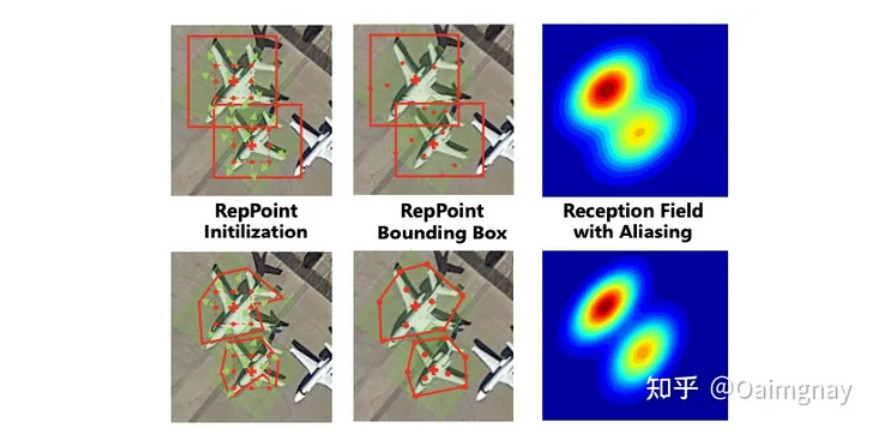
\includegraphics[width=400px]{./compare_cfa_with_other.JPG}
		\caption{Minh hoạ vấn đề. (Bên trên) Sử dụng cách biểu diễn dạng hộp, so với cách biểu diễn bao lồi (Bên dưới), hiện tương răng cưa đã được xử lý}
		\label{fig_dhandang1}
	\end{center}
\end{figure} 


Để giải quyết các vấn đề trên, một phương pháp đã được đưa ra đó là: phương pháp thích ứng bao lồi (convex-hull feature adaptation - CFA), hay \textit{bộ phát hiện CFA}. CFA được thực hiện dựa trên nguyên tắc biểu diễn bao lồi, định nghĩa một tập các điểm đặc trưng, giới hạn phạm vi của đối tượng mục tiêu nhờ sử dụng chỉ số CIoU. Bộ phát hiện này đạt được sự phân bổ đặc trưng tối ưu nhờ vào việc xây dựng tập bao lồi, cũng như phân chia linh hoạt các bao lồi thành các bao lồi âm và bao lồi dương. Ngoài ra, CFA xem xét sự chồng chéo nhau giữa bao lồi dự đoán và bao lồi thực tế, tiến hành phạt các bao lồi được chia sẻ bởi nhiều đối tượng, từ đó giúp giảm thiểu hiện tượng đặc trưng răng cưa (feature aliasing), đạt được sự thích ứng đặc trưng tối ưu. Bộ phát hiện đã đạt được kết quả tốt nhất khi thử nghiệm trên tập dữ liệu DOTA và SKUR110KR.

Phương pháp CFA được chia làm 2 giai đoạn thực hiện:
\begin{itemize}
	\item Giai đoạn 1: tạo tập bao lồi, ước lượng sơ bộ bố cục của bao lồi.
	\item Giai đoạn 2: chỉnh sửa bao lồi để khớp với các đối tượng phân bổ dày đặc.
\end{itemize}

\begin{figure}[ht!]
	\begin{center}
		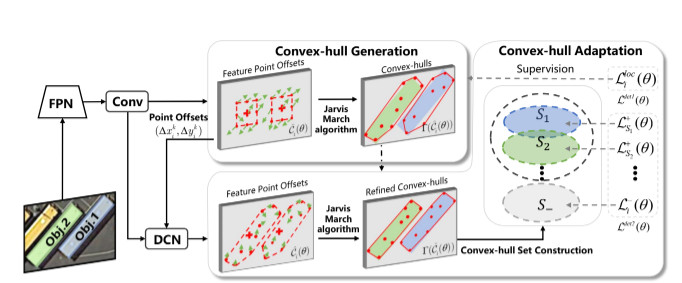
\includegraphics[width=450px]{./work_flow_cfa.JPG}
		\caption{Biểu đồ luồng quy trình thực hiện của bộ phát hiện CFA.}
		\label{work_flow_cfa}
	\end{center}
\end{figure} 

\section{Xây dựng tập bao lồi đầu tiên}
Thông thường, các hộp bao (bounding-box) dùng cho việc phát hiện đối tượng sử dụng hình chữ nhật để biểu diễn. Điều này đôi khi làm giảm khả năng biểu diễn đối tượng, do không phải đối tượng nào cũng có dạng hình chữ nhật. Chính vì thế, phương pháp CFA đã đề xuất biểu diễn phạm vi của đối tượng bằng bao lồi, giúp cho việc phát hiện đối tượng được hiệu quả hơn.\\
Mỗi bao lồi (convex-hull) là một tập hợp các điểm thoả mãn công thức:

\begin{align} \label{convex_hull_definition}
		C_i=\left\{\left(x_i^k, y_i^k\right)\right\}_i^{k=1 \ldots K}
\end{align}
Trong đó:
	\\ \indent	 $C_i$: bao lồi thứ i,
	\\ \indent	 $\left(x_i^k, y_i^k\right)$: điểm nằm trên bao lồi thứ k, với k là chỉ số của điểm đặc trưng, 
	\\ \indent	$K = 9$: tương ứng với 9 điểm được khởi tạo từ đầu cho mỗi bao lồi.

\begin{figure}[ht!]
	\begin{center}
		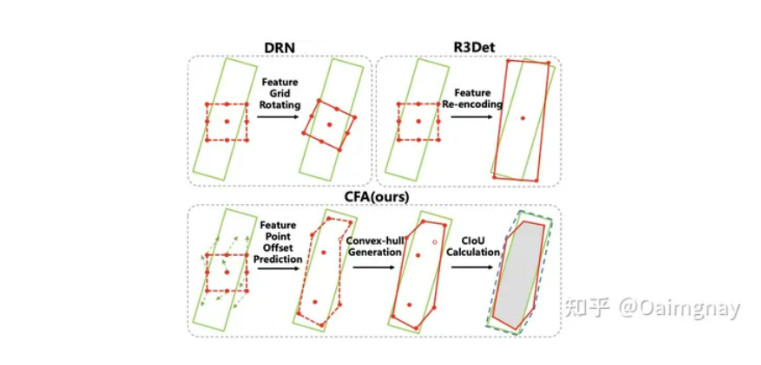
\includegraphics[width=445px]{./compare_convex-hull_with_rectangle.jpg}
		\caption{So sánh biểu diễn hộp có hướng (bên trên) so với biểu diễn bao lồi (ở dưới).}
	\end{center}
\end{figure} 


Việc huấn luyện có thể xem như là quá trình dự đoán độ lệch (offset), trong khi hệ số CIoU cần được tối đa hoá để đạt được so khớp tối ưu nhất. \\
Dưới đây là phương pháp sử dụng phép toán tích chập để dự đoán độ lệch:
$\left(\Delta x_i^k, \Delta y_i^k\right)$
với từng điểm đặc trưng, trả về một bản đồ phần bù các đặc trưng
$O \in R^{H \times W \times W}$ ($H, W, C$ lần lượt là chiều dài, chiều rộng và số kênh của bản đồ đặc trưng):
\begin{align} \label{convex_hull_learn_offset}
	\hat{\mathcal{C}}_i(\theta) \leftarrow\left\{\left(x_i^k+\Delta x_i^k(\theta), y_i^k+\Delta y_i^k(\theta)\right)\right\}_i^{k=1 \ldots K}
\end{align}

\indent$\theta$ được ký hiệu là các tham số của mạng.

\section{Tích chập biến dạng}
Tích chập biến dạng (Deformable convolution - DCN) \cite{dai17dcn} là dạng tích chập mà vị trí thực hiện tích chập bị biến dạng, không giống tích chập truyền thống là dạng lưới $N\mathrm{x}N$. Ưu điểm của phương pháp này giúp trích xuất các đặc trưng mong muốn được chính xác hơn, lấy mẫu được ở những vị trí đa dạng hơn (Phép tích chập truyền thống chỉ có thể trích xuất các đặc trưng trên một khung hinh chữ nhật).(Hình \ref{so_sanh_tich_chap_thong_thuong_deformable})

\begin{figure}[ht!]
	\begin{center}
		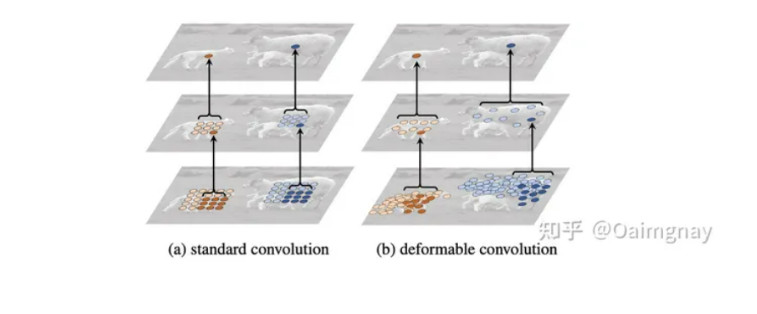
\includegraphics[width=445px]{./compare_normal_with_deformable_convolution.jpg}
		\caption{So sánh tích chập thông thường và tích chập biến dạng.}
		\label{so_sanh_tich_chap_thong_thuong_deformable}
	\end{center}
\end{figure} 

Phép tích chập biến dạng thực ra là thêm phần bù cho các điểm tích chập lấy mẫu. (Hình \ref{offset_deformable_convolution})

\begin{figure}[ht!]
	\begin{center}
		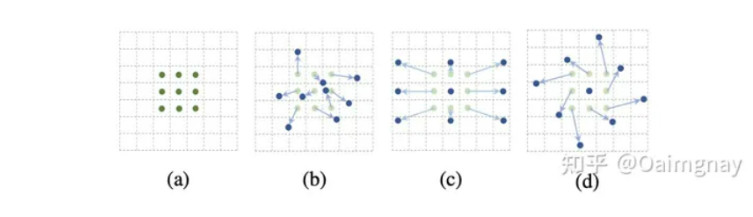
\includegraphics[width=445px]{./feature_offset_type.jpg}
		\caption{Các phép biến đổi tích chập biến dạng khác nhau
		}
		\label{offset_deformable_convolution}
	\end{center}
\end{figure} 

\begin{figure}[ht!]
	\begin{center}
		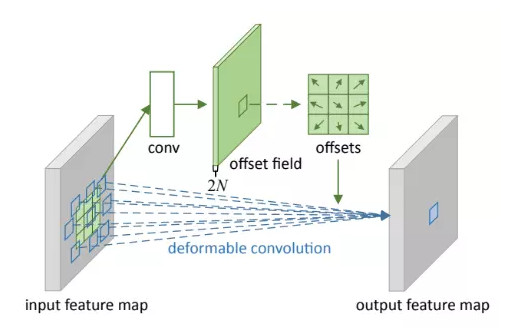
\includegraphics[width=400px]{./deformable_process.jpg}
		\caption{Quá trình thực hiện tích chập biến dạng.}
		\label{deformable_process}
	\end{center}
\end{figure} 


Cho đầu vào là một bản đồ đặc trưng, giả sử phép tích chập là 3x3. Để học được phần bù, định nghĩa một lớp tích chập 3x3 khác, chiều của đầu ra là kích thước của bản đồ đặc trưng ban đầu, số kênh = $2N$. (Hình \ref{deformable_process}) Tiếp theo thực hiện tích chập biến dạng, dựa trên độ bù của các phần đã được tính trước đó, sau đó thực hiện phép tích chập như thông thường.
\section{Thuật toán tìm bao lồi}
Sau khi học được phần bù, CFA cập nhật các điểm đặc trưng của bao lồi, được thực hiện bởi thuật toán Jarvis March. Kết quả là bao lồi nhỏ nhất phù hợp điều kiện sẽ được chọn ra sau mỗi lần lặp.

\subsection{Thuật toán Jarvis March}





\subsection{Thuật toán Outer Convex Approximation}
\begin{figure}[ht!]
	\begin{center}
		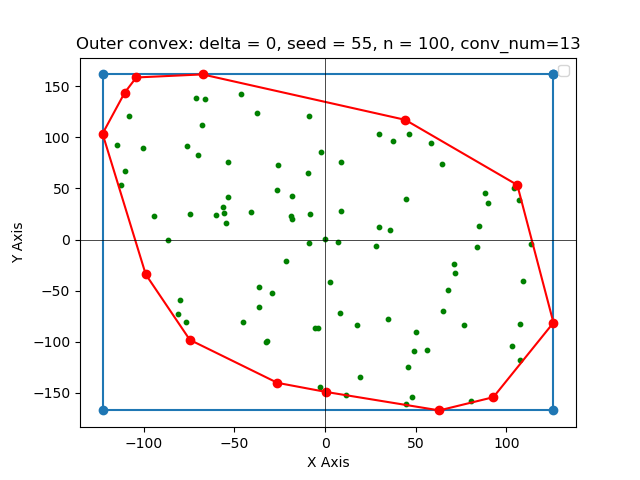
\includegraphics[width=350px]{./outer_convex_approximation_brief.png}
		\caption{Minh họa thuật toán Outer Convex Approximation.}
		\label{outer_convex_approximation_brief}
	\end{center}
\end{figure} 
Tóm tắt thuật toán: Xuất phát từ một hình chữ nhật nhỏ nhất bao quanh tất cả các điểm (màu xanh dương), duyệt lần lượt các đỉnh được chọn, xác định hướng cực đại (direction) nhờ hai điểm liền trước (predecessor) và điểm liền sau (successor), tính toán theo công thức để quyết định việc lấy thêm đỉnh mới cho bao lồi hay không. Kết quả cuối cùng sẽ là hình chữ nhật được cải thiện dần thành bao lồi (màu đỏ) phù hợp với toàn bộ tập điểm (Hình \ref{outer_convex_approximation_brief}). 
\subsection{Inner Convex Approximation}

Tóm tắt thuật toán): Xuất phát từ hình tứ giác ban đầu (màu cam), xét mỗi cạnh của đa giác, chọn các điểm phù hợp trong tập điểm nằm phía trên cạnh, từ đó xem xét có nên thêm cạnh mới hay không, nhằm mở rộng tứ giác ban đầu. Sau cùng khi không còn điểm nào nằm phía trên các cạnh, thuật toán sẽ kết thúc và trả về bao lồi kết quả(màu xanh lam). (Hình \ref{inner_convex_brief}).

\begin{figure}[ht!]
	\begin{center}
		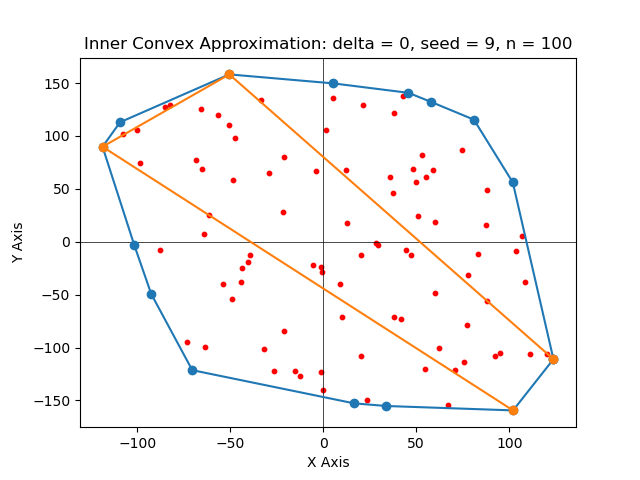
\includegraphics[width=350px]{./inner_convex_brief.png}
		\caption{Minh họa thuật toán Inner Convex Approximation với đầu vào gồm 100 điểm ngẫu nhiên.}
		\label{inner_convex_brief}
	\end{center}
\end{figure} 
\section{Đinh nghĩa công thức Convex Intersection over Union (CIoU)}
Dựa vào mỗi bao lồi dự đoán, ta tính toán được hàm mất mát vị trí (localization) và phân lớp (classification)của một đối tượng. Công thức CIoU giữa bao lồi dự đoán thứ $i$:  $C_i(\theta)$ và bao lồi thực tế $\mathcal{B}_j$ của đối tượng thứ $j$ được tính như sau:

\begin{align} \label{CioU_fomular}
	\operatorname{CIoU}\left(\mathcal{C}_i(\theta), \mathcal{B}_j\right)=\frac{\left|\mathcal{C}_i(\theta) \cap \mathcal{B}_j\right|}{\left|\mathcal{C}_i(\theta) \cup \mathcal{B}_j\right|}-\frac{\left|\mathcal{R}_j \backslash\left(\mathcal{C}_i(\theta) \cup \mathcal{B}_j\right)\right|}{\left|\mathcal{R}_j\right|}
\end{align}
Trong đó, $\mathcal{R}_j$ là đa giác nhỏ nhất có thể bao quanh  $C_i(\theta)$ và $\mathcal{B}_j$.
\section{Hàm mất mát}
Theo công thức (\ref{CioU_fomular}), hàm mất mát vị trí CIoU được định nghĩa là:
\begin{align} \label{cong_thuc_ham_loss_CIoU}
	\mathcal{L}_i^{l o c}(\theta)=1-\operatorname{CIoU}\left(\mathcal{C}_i(\theta), \mathcal{B}_j\right)
\end{align}
Cho $f_i^{k}(\theta)$ là đặc trưng của điểm thứ $k$, bao lồi đặc trưng $f_i(\theta)$ được tính bởi tổng có trọng số của tất cả các điểm đặc trưng trên bao lồi dự đoán $\mathcal{C}_i(\theta)$, tức là bằng công thức: $f_i(\theta) = \sum_{k}m w_i^k.f_i^k(\theta)$, trong đó, $w_i^k$ biểu thị các trọng số đặc trưng có thể học được từ tích chập biến dạng (DCN). Dựa vào bao lồi đặc trưng, điểm dự đoán $S_i(\theta)$ của bao lồi dự đoán $C_i(\theta)$ được tính bởi phép tích chập, hàm mất mát phân loại của bao lồi dự đoán $C_i(\theta)$ tương ứng với $B_j$ được định nghĩa là:
\begin{align} \label{loss_classification}
	\mathcal{L}_i^{c l s}(\theta)=\mathrm{FL}\left(S_i(\theta), Y_j\right)
\end{align}
Trong đó, $Y_j$ biểu thị là nhãn nhị phân thật sự (ground-truth) và FL() là hàm mất mát Focal (Focal loss). Kết quả thu được là hàm mất mát của bao lồi dương: 
\begin{align} \label{loss_function_positive_convex}
	\mathcal{L}_i^{+}(\theta)=\mathcal{L}_i^{c l s}\left(\mathcal{S}_i(\theta), Y_j\right)+\lambda \mathcal{L}_i^{l o c}\left(\mathcal{C}_i(\theta), \mathcal{B}_j\right)
\end{align}
Hàm mất mát (\ref{loss_function_positive_convex}) là tổng của hàm mất mát vị trí (\ref{cong_thuc_ham_loss_CIoU}) và hàm mất mát phân loại (\ref{loss_classification}). Tương tự ta có hàm mất mát dành cho bao lồi âm:

\begin{align} \label{loss_negative_convex}
	\mathcal{L}_i^{-}(\theta)=\mathcal{L}_i^{c l s}\left(\mathcal{S}_i(\theta), Y_j\right)
\end{align}
Trong quá trình huấn luyện, vì các bao lồi được ban đầu chỉ được sinh ra bằng cách tối ưu CIoU, nên cần định nghĩa một hàm loss cho việc giám sát:
\begin{align} \label{loss_det_1}
	\mathcal{L}^{\operatorname{det} 1}(\theta)=\frac{1}{J} \sum_i \mathbb{I}_{\left(x_i, y_i\right)} \mathcal{L}_i^{l o c}(\theta)
\end{align}
Nói tóm lại, trong giai đoạn đầu tiên của việc sinh bao lồi, hàm mất mát $L^{\operatorname{det} 1}$ bên trên là hàm cần được xem xét. Trong giai đoạn 2, hai hàm mất mát phân lớp (\ref{loss_negative_convex}) và (\ref{loss_function_positive_convex}) sẽ được sử dụng để phân loại bao lồi.
\section{Thích ứng bao lồi}
Phương pháp biểu diễn bằng bao lồi giúp định vị đối tượng ở bất kỳ hình dạng nào. Tuy nhiên vẫn xảy ra một vấn đề, đó là làm thế nào để định vị một cách chính xác các đối tượng dày đặc, đặc biệt là các đối tượng có đặc trưng răng cưa (feature aliasing). Chính vì thế, bộ phát hiện CFA đã đề xuất một phương pháp thích ứng mới, giúp tinh chỉnh các bao lồi trong ở giai đoạn 1 để thu được vị trí chính xác hơn và phân lớp hiệu quả hơn.
\subsection{Xây dựng tập các bao lồi}
CFA xây dựng một tập các bao lồi với mỗi đối tượng, để một đối tượng mục tiêu có thể khớp với nhiều bao lồi phù hợp, từ đó cùng nhau tối ưu các đặc trưng của các đối tượng dày đặc.

\begin{figure}[ht!]
	\begin{center}
		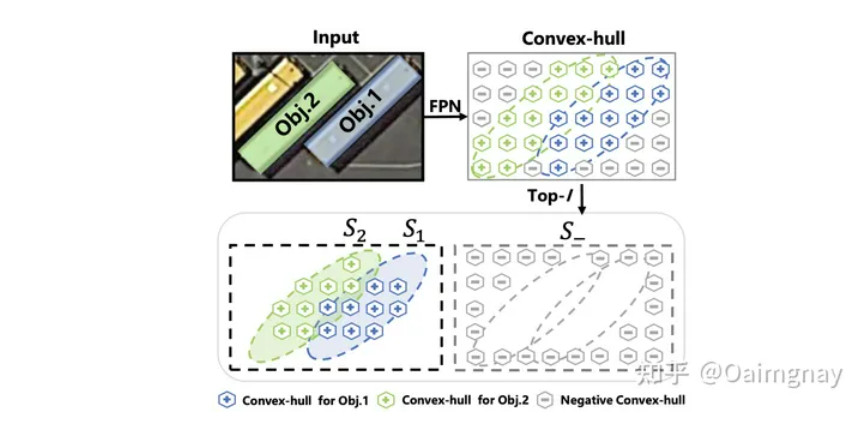
\includegraphics[width=445px]{./construction_convex_hull_set.jpg}
		\caption{Minh họa xây dựng tập các bao lồi để biểu diễn các đối tượng, đặc biệt với những đối tượng phân bổ dày đặc.}
		\label{fig_dhandang1}
	\end{center}
\end{figure} 
Với mỗi một đối tượng, việc xây dựng tập bao lồi tương ứng là: xem xét hệ số CIoU giữa bao lồi dự đoán và bao lồi thực tế, chọn ra top-\textit{I} bao lồi làm bao lồi dương để xây dựng tập các bao lồi. Các bao lồi còn lại không thuộc vào bất kỳ tập bao lồi nào sẽ được gộp lại thành tập bao lồi âm $S$.
\begin{align} \label{construct_convex_hull_set}
\mathcal{L}_{S_j}^{+}(\theta)=\frac{1}{\left|S_j\right|} \sum_{i \in S_j} \omega_i \mathcal{L}_i^{+}(\theta)
\end{align}
Khi nhiều đối tượng trong ảnh nằm gần nhau, không phải tất cả các bao lồi nằm trong tập bao lồi đều phù hợp với đối tượng. Các bao lồi có đặc trưng răng cưa sẽ phải được phân loại thành tập các bao lồi âm. Các bao lồi được chia sẻ bởi nhiều đối tượng thì sẽ có độ tin cậy thấp hơn các bao lồi khác.
\subsection{Chiến lược phân đoạn tập các bao lồi}
Để giải quyết vấn đề đặc trưng răng cưa ở các đối tượng dày đặc, bộ phát hiện CFA đề xuất chiến lược phân đoạn tập các bao lồi để đánh giá động các mẫu bao lồi âm và mẫu dương, chuyển đổi trọng số $\omega_i$ thành $f\left(L_i^{+}(\theta)\right)$. Sau khi thay thế, được công thức sau:
\begin{align} \label{loss_positive_convert}
	\mathcal{L}_{s_j}^{+}(\theta)=\frac{1}{\left|S_j\right|} \sum_{i \in S_j} f\left(\mathcal{L}_i^{+}(\theta)\right) \mathcal{L}_i^{+}(\theta)
\end{align}
Trong đó: $f$ là hàm lỗi đơn điệu giảm phân phối Gaussian: $f\left(x\right) = 1.0 - \frac{2}{\sqrt{\pi}}\int_0^xe^{-t^2}$, có nghĩa là giá trị mất càng nhỏ, độ tin cậy càng cao.

\begin{figure}[ht!]
	\begin{center}
		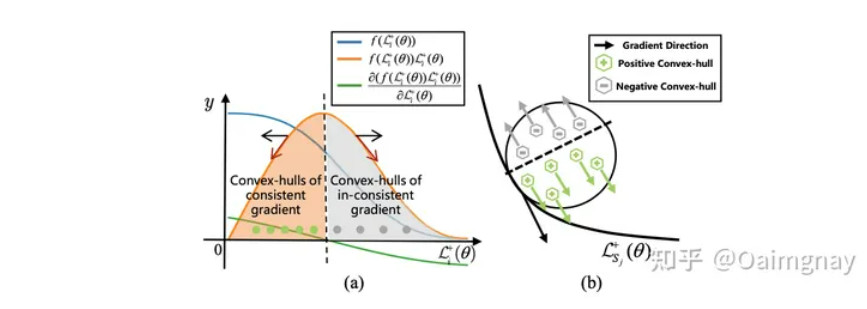
\includegraphics[width=445px]{./gaussian_gradient.jpg}
		\caption{Phân chia tập bao lồi theo hướng dẫn của nguyên tắc nhất quán độ dốc.}
		\label{gradient_consistentcy_illustration}
	\end{center}
\end{figure} 
Nguyên tắc phân chia tập bao lồi là nguyên tắc nhất quá độ dốc. Bằng cách lấy đạo hàm của công thức công thức \ref{loss_positive_convert}, ta có được:
\begin{align} \label{gradient_of_loss}
	 \frac{\partial \mathcal{L}_{s_j}^{+}(\theta)}{\partial \theta}=\frac{1}{\left|S_j\right|} \sum_{i \in S_j} \frac{\partial\left(f\left(\mathcal{L}_i^{+}(\theta)\right) \mathcal{L}_i^{+}(\theta)\right)}{\partial \mathcal{L}_i^{+}(\theta)} \frac{\partial \mathcal{L}_i^{+}(\theta)}{\partial \theta}
\end{align}
 Đạo hàm của mỗi một bao lồi dương $\frac{\partial L_i^{+}(\theta)}{\partial \theta}$ yêu cầu đạo hàm của toàn bộ tập bao lồi $\frac{\partial L_{S_j}^{+}(\theta)}{\partial \theta}$ là nhất quán, nghĩa là: bao lồi nào có độ dốc không nhất quán được xem là bao lồi âm. Những bao lồi này sẽ dẫn đến hiện tượng răng cưa đặc trưng. Xét công thức (\ref{gradient_of_loss}), nếu $\frac{\partial\left(f\left(L_i^{+}(\theta)\right) L_i^{+}(\theta)\right)}{\partial L_i^{+}(\theta)}$ mang giá trị dương, thì bao lồi $C_i$ được xếp là bao lồi dương, hoặc sẽ là bao lồi âm. Xem xét hình \ref{gradient_consistentcy_illustration}, khi sắp xếp các giá trị mất mát  $\frac{\partial L_i^{+}(\theta)}{\partial \theta}$ theo thứ tự tăng dần, $f\left(\partial L_i^{+}(\theta)\right) L_i^{+}(\theta)$ (đường màu cam) là một hàm lồi hướng lên với một cực trị duy nhất, trong khi đường  $\frac{\partial\left(f\left(L_i^{+}(\theta)\right) L_i^{+}(\theta)\right)}{\partial L_i^{+}(\theta)}$ (màu xanh lục) chia các bao lồi thành tập các bao lồi dương $S_j$ và tập bao lồi âm $S\_$.

Cùng lúc đó, để xử lý đặc trưng răng cưa, CFA cũng giới thiệu hệ số chống đặc trưng răng cưa:
\begin{align}\label{FAA_fomular}
	p_i = \gamma\dot{\frac{\mathrm{CIoU}(\mathcal{C}_i, \mathcal{B}_j)}{\sum_{m=1}^{M}\mathrm{CIoU}\left(\mathcal{C}_i, \mathcal{B}_j\right)}}
\end{align}
Hệ số này thể hiện mức độ mà một đối tượng thuộc về một đối tượng duy nhất, khi nó chồng lên M đối tượng khác. $\gamma$ là hệ số chống đặc trưng răng cưa.
Hàm mất mát được cập nhật thành: 

\begin{align}\label{loss_update}
	\mathcal{L}_{s_j}^{+}(\theta)=\frac{1}{\left|S_j\right|} \sum_{i \in S_j} p_i f\left(\mathcal{L}_i^{+}(\theta)\right) \mathcal{L}_i^{+}(\theta)
\end{align}
Nói tóm lại, giai đoạn 2 của quá trình tối ưu được điều khiển bởi hàm mất mát trên tập bao lồi, được xác định bằng cách kết hợp hàm mất mát phân loại và hàm mất mát vị trí:
\begin{align} \label{loss_det_2}
	\begin{aligned}
		\mathcal{L}^{\operatorname{det} 2}(\theta)= & \frac{1}{J} \sum_{j=1}^J \frac{1}{\left|S_j\right|} \sum_{i \in S_j} p_i f\left(\mathcal{L}_i^{+}(\theta)\right) \mathcal{L}_i^{+}(\theta) \\
		& +\frac{1}{\left|S_{-}\right|} \sum_{i \in S_{-}} \mathcal{L}_i^{-}(\theta)
	\end{aligned}
\end{align}

Hàm mất mát này xem xét sự tương ứng về đặc trưng của nhiều đối tượng, tiến hành phạt các bao lồi được chia sẻ bởi nhiều đối tượng, và giảm thiểu đặc trưng răng cưa để đạt được thích ứng đặc trưng tối ưu. Cuối cùng hàm mất mát của toàn bộ bộ phát hiện CFA là: 
\begin{align} \label{final_loss_CFA}
	L^{\operatorname{det} 1}(\theta)+L^{\operatorname{det} 2}(\theta)
\end{align}
Tóm lại trong chương 1 trình bày lý thuyết của bộ phát hiện CFA, bao gồm cách biểu diễn hộp bao bằng bao lồi, thuật toán tìm bao lồi, hàm loss CIoU và cách thích ứng đặc trưng của bộ phát hiện sử dụng chiến lược phân chia tập các bao lồi.
\chapter{Thuật toán tính bao lồi xấp xỉ}
Thuật toán tìm bao lồi xấp xỉ nhận đầu vào là một tập các điểm ngẫu nhiên, đầu ra trả về một tập điểm biểu diễn một bao lồi bao quanh tất cả các điểm còn lại. Với ngưỡng $\delta$ tuỳ chỉnh, sẽ cho ra được dạng bao lồi khác nhau.
\section{Outer convex approximation}
Cho tập X được định nghĩa như sau:
\begin{align} \label{ct2.1} 
	X:=\left\{x_1, x_2, \ldots, x_n\right\} \subset \mathbb{R}^2
\end{align}
Giả sử không mất tính tổng quát rằng:
\begin{align} \label{ct2.2} 
	x_1, x_2, \ldots, x_n  \text{ không cùng nằm trên cùng một đường thẳng.}
\end{align}
Ta viết tất cả các vector thành dạng vector hàng, những vector này sẽ có chuyển vị của chúng được ký hiệu bởi chỉ số trên $T$, và sử dụng chỉ số trên để chỉ định các thành phần của chúng, ví dụ: $x = \left(x^1, x^2\right)\in\mathbb{R}^2$. Cho $x, x'\in\mathbb{R}^2$, chứng tỏ:
\begin{equation}\label{ct2.3}
	\begin{aligned}
		& {\left[x, x^{\prime}\right]:=\left\{(1-\lambda) x+\lambda x^{\prime} \mid \lambda \in[0,1]\right\}} \\
		& \left(x, x^{\prime}\right):=\left\{(1-\lambda) x+\lambda x^{\prime} \mid \lambda \in(0,1)\right\}
	\end{aligned}
\end{equation}

Cho $X$ thỏa mãn (\ref{ct2.1}) - (\ref{ct2.2}) và $\delta \geq 0$, trong phần này ta muốn tìm một bao lồi xấp xỉ của $X$, ký hiệu:
\begin{align}\label{ct2.4}
	\text{Đa giác lồi }\mathcal{P}^{outer} \text{thỏa mãn bao lồi }X\subset\mathcal{P}^{outer}
\end{align}
sao cho:
\begin{align}\label{ct2.5}
	dist_H\left(conv\ X, \mathcal{P}^{outer}\right) \leq \delta
\end{align}
$\mathcal{P}^{outer}$ đươc xác định bởi:
\begin{align}\label{ct2.6}
	\mathcal{P}^{outer} := \{x\in\mathbb{R}^2 |\ dx^T \leq \beta_d\ \text{ với tất cả d} \in D\}
\end{align}
Trong đó $D \subset \mathbb{R}^2$ biểu thị tập các hướng tối đa, $\beta_d \in \mathbb{R}$ biểu thị ngưỡng tương ứng với hướng $d \in D$. Với tập D cho trước, $\mathcal{P}^{outer}$ là bao lồi xấp xỉ phù hợp nhất chứa $X$ nếu như:
\begin{equation}\label{ct2.7}
	\beta_d:=\max _{x \in X}\ d x^T \text{với tất cả d }\in D
\end{equation}
Cho P là tập các đỉnh của $\mathcal{P}^{outer}$.\\
Ta bắt đầu quá trình xác định bao lồi xấp xỉ ngoài với hình chữ nhật nhỏ nhất chứa $X$, có chứa cạnh song song với trục tung và trục hoành. Theo công thức (\ref{ct2.5}) - (\ref{ct2.6}), hình chữ nhật $\mathcal{P}^{outer}$ được xác định như sau:
\begin{align}\label{ct2.8}
	D:=\{(1, 0), (0, 1), (-1, 0), (0, -1)\}
\end{align}
và:
\begin{equation}\label{ct2.9}
	\begin{aligned}
		& \beta_{(1,0)}:=\max \left\{x^1 \mid\left(x^1, x^2\right) \in X\right\}, \\
		& \beta_{(0,1)}:=\max \left\{x^2 \mid\left(x^1, x^2\right) \in X\right\}, \\
		& \beta_{(-1,0)}:=\max \left\{-x^1 \mid\left(x^1, x^2\right) \in X\right\}, \\
		& \beta_{(0,-1)}:=\max \left\{-x^2 \mid\left(x^1, x^2\right) \in X\right\} .
	\end{aligned}
\end{equation}
Theo công thức (\ref{ct2.2}) ta có:

\begin{center}
	$\beta_{(-1, 0)} \textless \beta_{(1, 0)}$ \text{ và } $\beta_{(0, -1)} \textless \beta_{(0, 1)}$
\end{center}
Vì vậy, $\mathcal{P}^{outer}$ là một hình chữ nhật phù hợp với 4 đỉnh phân biệt, có tập đỉnh là:
\begin{align}\label{ct2.10}
	P := \{r_1, r_2, r_3, r_4\}
\end{align}
Trong đó:
\begin{equation}\label{ct2.11}
	\begin{aligned}
		& r_1:=\left(\beta_{(1,0)}, \beta_{(0,1)}\right), \\
		& r_2:=\left(\beta_{(-1,0)}, \beta_{(0,1)}\right), \\
		& r_3:=\left(\beta_{(-1,0)}, \beta_{(0,-1)}\right), \\
		& r_4:=\left(\beta_{(1,0)}, \beta_{(0,-1)}\right) .
	\end{aligned}
\end{equation}
Trong các bước xấp xỉ tiếp theo, xây dựng đa giác $\mathcal{P}^{outer}$ được cải thiện dần dần như sau:

$\text{Với mỗi }p \in P, \text{lấy } p^{-} \in P \text{ và } p^{+} \in P \text{ lần lượt là}$
\begin{align} \label{ct2.12}
\text {điểm liền trước ngược chiều kim đồng hồ và điểm liền sau của } p.
\end{align}
Xét công thức sau:
\begin{equation}\label{ct2.13}
	\begin{array}{lcl}
		d_{p}^T &:=& \|p^+ - p^-\|^{-1}\, R \, (p^+ - p^-)^T, \\
		\beta_{d_{p}} &:=& \max\{d_{p}\, x^T \mid x \in X\},
	\end{array}
\end{equation}
Trong đó:
\begin{equation}\label{ct2.14}
	R := \begin{pmatrix}
		0 & -1 \\
		1 & 0
	\end{pmatrix}
\end{equation}
là ma trận xoay ngược chiều theo hướng kim đồng hồ với góc xoay $\pi/2$. Vì $R$ là ma trận xoay, ta có:
\begin{equation}\label{ct2.15}
	\|d_{p}\| = \|p^+ - p^-\|^{-1}\, \|(p^+ - p^-) R^T\| = \|p^+ - p^-\|^{-1}\, \|p^+ - p^-\| = 1.
\end{equation}
Có hai trường hợp xảy ra khi ta thêm các ràng buộc tuyến tính sau vào định nghĩa của $\mathcal{P}^{outer}$ trong công thức (\ref{ct2.6}):
\begin{equation}\label{ct2.16}
	d_p\, x^T \leq \beta_{d_p}.
\end{equation}

Trường hợp 1, nếu:
\begin{equation}\label{ct2.17}
	\beta_{d_p} = d_p\, p^+
\end{equation}
thì công thức (\ref{ct2.15}) sẽ không tạo thêm đỉnh mới mà thêm cạnh mới  $[p^-, p^+]$ vào ${\cal P}^{\rm outer}$. Xét $d_{[p^-, p]}$ và $d_{[p, p^+]}$ là 2 hướng cực đại trong D, định nghĩa hai cạnh $[p^-, p]$ và $[ p, p^+]$ của ${\cal P}^{\rm outer}$. Sau đó $d_{[p^-, p]}$ and $d_{[p, p^+]}$ sẽ trở nên vô dụng. Vậy nên khi thêm $d_p$ vào tập $D$ cần phải loại bỏ $d_{[p^-, p]}$ và đỉnh $d_{[p, p^+]}$ và $p$ trong $P$:
\begin{equation}\label{ct2.18}
	\begin{array}{lcl}
		D &:=& (D \cup \{d_{p}\})\setminus \{d_{[p^-,p]}, d_{[p,p^+]}\}, \\
		P &:=& P \setminus \{p\}.
	\end{array}
\end{equation}
Trường hợp 2, nếu
\begin{equation}\label{ct2.19}
	\beta_{d_p} > d_p\, p^+
\end{equation}
và:
\begin{equation}\label{ct2.20}
	d_{p}\, p^T - \beta_{d_{p}} > \delta
\end{equation}
thì ràng buộc (\ref{ct2.16}) tạo ra hai đỉnh mới của ${\cal P}^{\rm outer}$ có tên $\hat p^-$ và $\hat p^+$, được tính như sau:
\begin{equation}\label{ct2.21}
	\begin{array}{lcl}
		\lambda_p &:=& (\beta_{d_p} - d_p\, p^{-T})/(d_p\, p^T - d_p\, p^{-T}) \in (0, 1), \\
		\hat p^- &:=& (1 - \lambda_p)\, p^{-T} + \lambda_p\, p^T, \\
		\hat p^+ &:=& (1 - \lambda_p)\, p^{+T} + \lambda_p\, p^T.
	\end{array}
\end{equation}

Ta thêm $d_p$ vào $D$ và thay $p \in P$ bởi $\hat p^-$ và $\hat p^+$:
\begin{equation}\label{ct2.22}
	\begin{array}{lcl}
		D &:=& D \cup \{d_{p}\}, \\
		P &:=&(P \setminus \{p\}) \cup \{\hat p^-, \hat p^+\}.
	\end{array}
\end{equation}

Quy trình thực hiện được mô tả bên dưới, trong đó $P_{\rm doubt}$ biểu thị tập hợp các đỉnh vẫn cần được kiểm tra.

\begin{algorithm}\label{alg01}  \rm 
		\floatname{algorithm}{Thuật toán}
		\caption{}  \label{al-blduoi0}
	\emph{Input:} Tập hữu hạn $X \subset \R^2$ và tham số xấp x $\delta \geq 0$. \\
	\emph{Output:} Đa giác xấp xỉ lồi ${\cal P}^{\rm outer}$ được xác định ở công thức (\ref{ct2.6}) bởi $D$ và $\beta_d$ cho $d \in D$ và tập đỉnh $P$.
	\begin{enumerate}
		\item\label{stepIalg01} 
		Xác định $D$, $\beta_d$ với $d \in D$, và $P$ theo (\ref{ct2.8})--(\ref{ct2.11}).
		
		\item\label{stepIIalg01} Đặt $P_{\rm doubt} := P$.
		
		\item\label{stepIIIalg01} 
		 Chọn một đỉnh bất kỳ $p \in P_{\rm doubt}$, tính toán $d_p$, $\beta_{d_p}$ theo (\ref{ct2.12})--(\ref{ct2.14}). \\
		Nếu (\ref{ct2.17}) là đúng thì thay đổi $D$, $P$ như (\ref{ct2.18}), thay đổi $P_{doubt}$ thành:
		\begin{equation}\label{ct2.23}
			P_{\rm doubt} := P_{\rm doubt} \setminus \{p, p^-, p^+\},
		\end{equation}
		sau đó chuyển sang bước \ref{stepIValg01}.\\
		Nếu % (\ref{betagreater}) and 
		(\ref{ct2.20}) là đúng, thay đổi $D$, $P$ như (\ref{ct2.22}), cập nhật:
		\begin{equation}\label{ct2.24}
			P_{\rm doubt} := (P_{\rm doubt} \setminus \{p\}) \cup \{\hat p^-, \hat p^+\},
		\end{equation}
		sau đó chuyển sang bước \ref{stepIValg01}.\\
		Nếu hai trường hợp trên không đúng thì, 
		\begin{equation}\label{ct2.25}
			P_{\rm doubt} := P_{\rm doubt} \setminus \{p\}.
		\end{equation}
		
		\item\label{stepIValg01} 
		Nếu $P_{\rm doubt} \ne \emptyset$  thì quay lại bước \ref{stepIIIalg01}.
		
		\item
		 Kết quả trả về tập hợp các hướng cực đại $D$ và $\beta_d$ với $d \in D$, tập đỉnh $P$ của ${\cal P}^{\rm outer}$, kết thúc thuật toán.
	\end{enumerate}
\end{algorithm}



\medskip
Bảng \ref{table02} cho thấy một số kết quả thử nghiệm, trong đó:
\begin{itemize}
	\item $\#_{\rm Vertices @ Alg.\, 1}$  là số cạnh trung bình của đa giác xấp xỉ lồi bao ngoài ${\cal P}^{\rm outer}$ được trả về bởi thuật toán 1,
	\item $\#_{\rm Step\, III @ Alg.\, 1}$ là số lần thực hiện trung bình của bước III của thuật toán 1.
\end{itemize}

\begin{table}[ht]
	\begin{center}\renewcommand{\arraystretch}{1.2}\small
		\setlength\tabcolsep{0.2cm}
		\begin{tabular}{|c|c||c|c|c|c|c|c|c|c|c|c|c|c|}
			%\hline
			\hline
			\multicolumn {2}{|c||}{\footnotesize $\#X=n$}  & 50 & 500 & 1000 & 2500 & 5000 & 7500\\ 
			\hline		
			\hline
			{ $\delta = 70$}
			
			& $\#_{\rm Edges@ Alg.\, 1}$  &5 & 5 & 5 & 5 & 5 & 5 \\
			
			& $\#_{\rm Step\, III @ Alg.\,1}$ &6 & 6 & 6 & 6 & 6 & 6   \\
			\hline
			{ $\delta = 10$}
			
			& $\#_{\rm Edges@ Alg.\,1}$  &11 & 11 & 14 & 13 & 11 & 11 \\
			
			& $\#_{\rm Step\, III @ Alg.\, 1}$&18 & 18 & 24 & 22 & 18 & 18\\
			\hline
			{ $\delta = 1$}
			
			& $\#_{\rm Edges@ Alg.\,1}$  &15 & 33 & 36 & 33 & 32 & 33 \\
			
			& $\#_{\rm Step\, III @ Alg.\, 1}$&38 & 70 & 70 & 62 & 60 & 64  \\
			\hline
			{ $\delta = 0$}
			
			& $\#_{\rm Edges@ Alg.\, 1}$  &12 & 23 & 30 & 38 & 43 & 43  \\
			
			& $\#_{\rm Step\, II @ Alg.\, 1}$&44 & 88 & 116 & 148 & 168 & 168  \\
			\hline
		\end{tabular}
		\caption{Số cạnh trung bình của đa giác lồi xấp xỉ lồi trong ${\cal P}^{\rm outer}$ trả về bởi thuật toán 1 và số lần thực hiện trung bình của bước 3 khi $X$ gồm $n$ điểm ngẫu nhiên trong đa giác có khung $16$ cạnh (Hình \ref{frame_polygon}).}
		\label{table03}
	\end{center}
\end{table} 	
\medskip
Bảng \ref{table02} thể hiện một số kết quả thực nghiệm về thời gian chạy của thuật toán Outer Convex Approximation khi $X$ gồm $n$ điểm ngẫu nhiên được trình bày trong bảng \ref{table02} phải được tạo ra trong đa giác có khung $16$ cạnh ${\cal P}^\diamond$ hiển thị trong hình \ref{frame_polygon}.

\begin{table}[ht]
	\begin{center}\renewcommand{\arraystretch}{1.2}\small
		\setlength\tabcolsep{0.05cm}
		\begin{tabular}{|c|c||c|c|c|c|c|c|c|c|c|}
			%\hline
			\hline
			\multicolumn {2}{|c||}{\footnotesize $\#X=n$} & 50 & 500 & 1000 & 2500 & 5000 & 7500 \\ 
			\hline		
			\hline
			{ $\delta = 70$}
			
			& $T_{\rm Alg.\, 1}$  &0.001531 & 0.001005 & 0.0 & 0.001025 & 0.000975 & 0.001025\\
			
			& $T_{\rm Alg.\, 1}/n$&3.06273e-05 & 2.0099e-06 & 0.0 & 4.102e-07 & 1.949e-07 & 1.367e-07 \\
			\hline
			{ $\delta = 10$}
			
			& $T_{\rm Alg.\, 3}$  &0.003005 & 0.003535 & 0.008002 & 0.006525 & 0.003 & 0.006528 \\
			
			& $T_{\rm Alg.\, 3}/n$&6.01006e-05 & 7.0691e-06 & 8.0023e-06 & 2.61e-06 & 6.001e-07 & 8.705e-07  \\
			\hline
			{ $\delta = 1$}
			
			& $T_{\rm Alg.\, 3}$  &0.012033 & 0.016051 & 0.014219 & 0.01155 & 0.013153 & 0.013655\\
			
			& $T_{\rm Alg.\, 3}/n$&0.0002406549 & 3.21026e-05 & 1.42186e-05 & 4.62e-06 & 2.6307e-06 & 1.8206e-06\\
			\hline
			{ $\delta = 0$}
			
			& $T_{\rm Alg.\, 3}$  &0.009627 & 0.019119 & 0.027318 & 0.036492 & 0.060799 & 0.054085 \\
			
			& $T_{\rm Alg.\, 3}/n$&0.0001925468 & 3.82371e-05 & 2.7318e-05 & 1.45967e-05 & 1.21599e-05 & 7.2113e-06\\
			\hline
		\end{tabular}
		\caption{Thời gian chạy trung bình $T_{\rm Alg.\,3}$  thuật toán \ref{al-blduoi4} khi $X$ gồm $n$ điểm ngẫu nhiên được trình bày trong bảng \ref{table03} phải được tạo ra trong đa giác có khung $16$ cạnh ${\cal P}^\diamond$ hiển thị trong hình \ref{frame_polygon}.}
		\label{table02}
	\end{center}
\end{table} 	

\begin{figure}[ht!]
	\begin{center}
		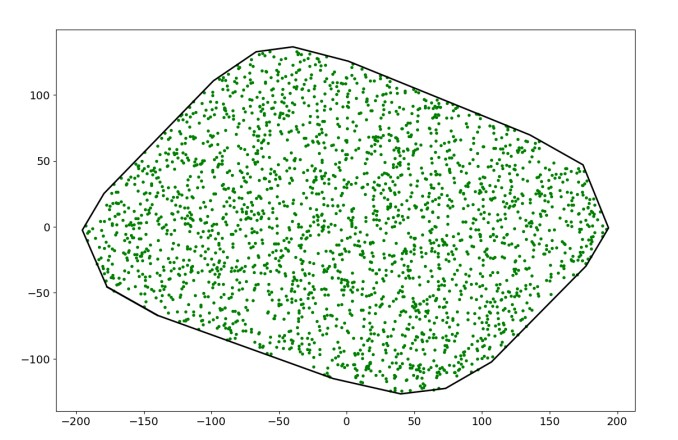
\includegraphics[width=350px]{./frame_polygon.jpg}
		\caption{Đa giác n điểm ngẫu nhiên có khung 16 cạnh ${\cal P}^\diamond$.}
		\label{frame_polygon}
	\end{center}
\end{figure} 	


Một vài hình ảnh kết quả chạy thuật toán Outer Convex Approximation với số điểm đầu vào bằng 100 được sinh ngẫu nhiên, và được đa giác 16 cạnh cắt thành tập các điểm nằm trong giới hạn kích thước nhỏ bao quanh mốc 150, với $\delta$ khác nhau (Hình \ref{outer_res_delta0}, \ref{outer_res_delta5}, \ref{outer_res_delta10}, \ref{outer_res_delta30}):
\begin{figure}[ht!]
	\begin{center}
		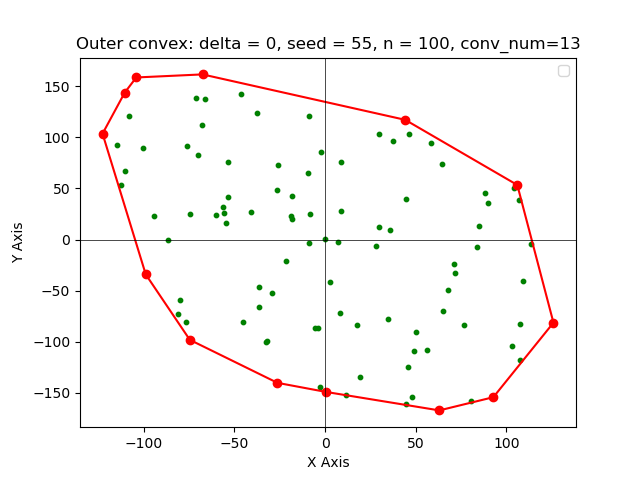
\includegraphics[width=350px]{./outer_res_delta0.png}
		\caption{Bao lồi kết quả khi chạy với $\delta$ = 0.}
		\label{outer_res_delta0}
	\end{center}
\end{figure} 	
\begin{figure}[ht!]
	\begin{center}
		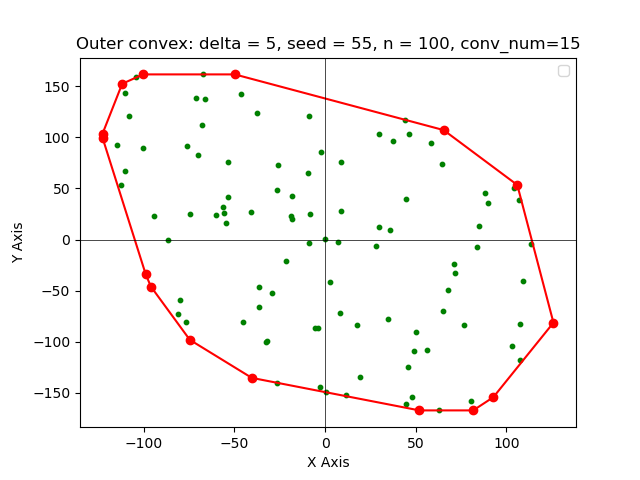
\includegraphics[width=350px]{./outer_res_delta5.png}
		\caption{Bao lồi kết quả khi chạy với $\delta$ = 5.}
		\label{outer_res_delta5}
	\end{center}
\end{figure} 	
\begin{figure}[ht!]
	\begin{center}
		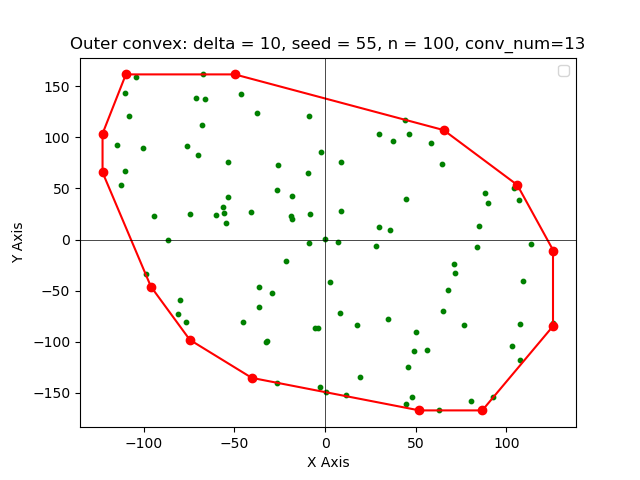
\includegraphics[width=350px]{./outer_res_delta10.png}
		\caption{Bao lồi kết quả khi chạy với $\delta$ = 10.}
		\label{outer_res_delta10}
	\end{center}
\end{figure} 	
\begin{figure}[ht!]
	\begin{center}
		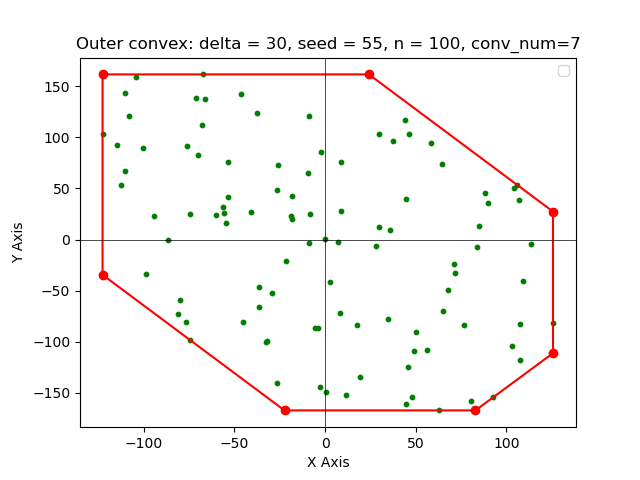
\includegraphics[width=350px]{./outer_res_delta30.png}
		\caption{Bao lồi kết quả khi chạy với $\delta$ = 30.}
		\label{outer_res_delta30}
	\end{center}
\end{figure} 	
\section{Inner convex approximation}\label{InnerConvexApproximation}

Cho $X$ thỏa mãn (\ref{ct2.1})--(\ref{ct2.2}) và $\delta \geq 0$. Ta sẽ tìm một bao lồi xấp xỉ trong ${\cal P}^{\rm inner}$ của $X$, tức là:
\begin{equation}\label{ct2.37}
	{\cal P}^{\rm inner} := \ conv X', \ \mbox{ với} X' \subset X,
\end{equation}
Sao cho:
\begin{equation}\label{ct2.38}
	\ dist_{\rm H}(\ conv X, {\cal P}^{\rm inner}) \leq \delta.
\end{equation}

Ta mô tả ${\cal P}^{\rm inner}$ bởi tập $E$ của các cạnh có hướng $[p, p^+]$, trong đó $p^+$  là đỉnh kế tiếp ngược chiều kim đồng hồ của $p$, tức là:
\begin{equation}\label{ct2.39}
	E := \{[p, p^+] \mid p, p^+ \in X', \mbox{ $[p, p^+]$ là một cạnh của ${\cal P}^{\rm inner}$}\}.
\end{equation}

Ta bắt đầu quá trình tìm bao lồi xấp xỉ trong với tứ giác $\bar q_1 \bar q_2 \bar q_3 \bar q_4$. Xét hai công thức sau:
\begin{equation}\label{ct2.40}
	\begin{array}{lcl}
		X' &:=& \{\bar q_1, \bar q_2, \bar q_3, \bar q_4\}, \\
		E &:=& \{[\bar q_1, \bar q_2], \, [\bar q_2, \bar q_3], \, [\bar q_3, \bar q_4], \, [\bar q_4, \bar q_1]\},
	\end{array}
\end{equation}
Trong đó $\bar q_1$, $\bar q_2$, $\bar q_3$, và $\bar q_4$ là độc nhất và được xác định bởi:
\begin{equation}\label{ct2.41}
	\begin{array}{lcl}
		x^1_{\rm min} &:=& \min \{x^1 \mid (x^1, x^2) \in X\}, \\
		x^1_{\rm max} &:=& \max \{x^1 \mid (x^1, x^2) \in X\}, \\
		x^2_{\rm min} &:=& \min \{x^2 \mid (x^1, x^2) \in X\}, \\
		x^2_{\rm max} &:=& \max \{x^2 \mid (x^1, x^2) \in X\}
	\end{array}
\end{equation}

\begin{equation}\label{ct2.42}
	\begin{array}{lcl}
		X^1_{\rm min} &:=& \{(x^1, x^2) \in X \mid x^1 = x^1_{\rm min}\}, \\
		X^1_{\rm max} &:=& \{(x^1, x^2) \in X \mid x^1 = x^1_{\rm max}\}, \\
		X^2_{\rm min} &:=& \{(x^1, x^2) \in X \mid x^2 = x^2_{\rm min}\}, \\
		X^2_{\rm max} &:=& \{(x^1, x^2) \in X \mid x^2 = x^2_{\rm max}\}
	\end{array}
\end{equation}
Và
\begin{equation}\label{ct2.43}
	\begin{array}{lcl}
		&& \bar q_1 = (\bar q_1^1, \bar q_1^2) \in X^1_{\rm max} \mbox{ thỏa mãn } \bar q_1^2 = \max\{x^2 \mid (x^1, x^2) \in X^1_{\rm max}\}, \\
		&& \bar q_2 = (\bar q_2^1, \bar q_2^2) \in X^2_{\rm max} \mbox{  thỏa mãn} \bar q_2^1 = \min\{x^1 \mid (x^1, x^2) \in X^2_{\rm max}\}, \\
		&& \bar q_3 = (\bar q_3^1, \bar q_3^2) \in X^1_{\rm min} \mbox{  thỏa mãn } \bar q_3^2 = \min\{x^2 \mid (x^1, x^2) \in X^1_{\rm min}\}, \\
		&& \bar q_4 = (\bar q_4^1, \bar q_4^2) \in X^2_{\rm min} \mbox{  thỏa mãn } \bar q_4^1 = \max\{x^1 \mid (x^1, x^2) \in X^2_{\rm min}\}.
	\end{array}
\end{equation}
Lưu ý rằng có thể hai trong số bốn điểm $\bar q_1$, $\bar q_2$, $\bar q_3$, và $\bar q_4$  trùng nhau, nhưng (\ref{ct2.2}) ngụ ý rằng phải ít nhất ba trong số chúng khác nhau.

Trong các bước tiếp theo, đa giác ${\cal P}^{\rm inner}$ được xây dựng và cải thiện 
như sau.\\
Xét cạnh bất kỳ $[p, p^+] \in E$ ($p \not= p^+$), xác định:
\begin{equation}\label{ct2.44}
	\begin{array}{lcl}
		\bar d_{[p, p^+]}^{\, T} &:=& \|p^+ - p\|^{-1} R \, (p^+ - p)^T, \\
		X_{[p, p^+]} &:=& \{x \in X \mid \bar d_{[p, p^+]}\, x^T > \bar d_{[p, p^+]}\, p^T \},
	\end{array}
\end{equation}
Với
\begin{equation*}%\label{rotationmatrix}
	R := \begin{pmatrix}
		0 & 1 \\
		-1 & 0
	\end{pmatrix}.
\end{equation*}

Nếu $X_{[p, p^+]} \not= \emptyset$ thì xác định:
\begin{equation}\label{ct2.45}
	\begin{array}{lcl}
		\beta_{[p, p^+]} &:=& \max \{\bar d_{[p, p^+]}\, x^T \mid x \in X_{[p, p^+]}\}, \\
		B_{[p, p^+]} &:=& \{x \in X_{[p, p^+]} \mid \bar d_{[p, p^+]}\, x^T = \beta_{[p, p^+]}\}.
	\end{array}
\end{equation}
Nếu:
\begin{equation}\label{dct2.46}
	\beta_{[p, p^+]} - \bar d_{[p, p^+]}\, p^T \leq \delta
\end{equation}
Thì không cần phải mở rộng ${\cal P}^{\rm inner }$ theo hướng $\bar d_{[p, p^+]}$ nữa.

Ngược lại, nếu:
\begin{equation}\label{ct2.47}
	\beta_{[p, p^+]} - \bar d_{[p, p^+]}\, p^T > \delta
\end{equation}
thì xác định điểm:
\begin{equation}\label{ct2.48}
	\hat p \in B_{[p, p^+]} \hbox{ thỏa mãn } \|\hat p - p\| = \max\{\|x - p\| \mid x \in B_{[p, p^+]}\},
\end{equation}
Và cập nhập $X'$ và $B$ bởi
\begin{equation}\label{ct2.49}
	\begin{array}{lcl}
		X' &:=& X' \cup \{\hat p\}, \\
		E &:=& E \cup \{[p, \hat p], \, [\hat p, p^+]\},
	\end{array}
\end{equation}
Và xác định: 
\begin{equation}\label{ct2.50}
	\begin{array}{lcl}
		X_{[p, \hat p]} &:=& \{x \in X_{[p, p^+]} \mid \bar d_{[p, \hat p]}\, x^T > \bar d_{[p, \hat p]}\, p^T \}, \\
		X_{[\hat p, p^+]} &:=& \{x \in X_{[p, p^+]} \mid \bar d_{[\hat p, p^+]}\, x^T > \bar d_{[\hat p, p^T]}\, {\hat p}^T \}.
	\end{array}
\end{equation}
Lưu ý rằng ta chỉ xem xét $x \in X_{[p, p^+]}$ trong định nghĩa này của $X_{[p, \hat p]}$ và $X_{[\hat p, p^+]}$, nhưng tất cả $x \in X$ đều được định nghĩa (\ref{ct2.44}) của $X_{[p, p^+]}$.

Quy trình tìm bao lồi được trình bày trong thuật toán sau, trong đó  $E_{\rm doubt}$ biểu thị tập hợp các cạnh cần được kiểm tra.

\begin{algorithm}\label{alg04}  \rm 
	\floatname{algorithm}{Thuật toán}
	\caption{}  \label{al-blduoi4}
	\emph{Input:} Tập hữu hạn $X \subset \R^2$ và tham số xấp xỉ $\delta \geq 0$. \\
	\emph{Output:} Đa giác lồi xấp xỉ trong ${\cal P}^{\rm inner}$ được mô tả bởi $X'$ và $E$.
	\begin{enumerate}
		\item\label{stepIalg04} 
		Tìm $X'$ và $E$ theo (\ref{ct2.40})--(\ref{ct2.43}).\\
		Với mọi ${[p, p^+]} \in E$ xác định $d_{[p, p^+]}$ và $X_{[p, p^+]}$ theo (\ref{ct2.44}).\\
		Cho $E_{\rm doubt} := E$.
		
		\item\label{stepIIalg04} 
		 Chọn một cạnh $[p, p^+] \in E_{\rm doubt}$. \\
		Nếu $X_{[p, p^+]} = \emptyset$, đặt
		$E_{\rm doubt} := E_{\rm doubt} \setminus \{[p, p^+]\}$
		và đi tới bước \ref{stepIIIalg04}.\\
		Tìm $\beta_{[p, p^+]}$ và $B_{[p, p^+]}$ theo (\ref{ct2.45}). \\
		Nếu (\ref{dct2.46}) đúng, đặt
		$E_{\rm doubt} := E_{\rm doubt} \setminus \{[p, p^+]\}$
		Và đi tới bước \ref{stepIIIalg04}.\\
		Trường hợp còn lại, lấy $\hat p$ định nghĩa theo (\ref{ct2.48}),
		 cập nhật $X'$ và $E$ theo (\ref{ct2.49}), và xác định $X_{[p, \hat p]}$ và $X_{[\hat p, p^+]}$ theo (\ref{ct2.50}), đặt
		\begin{equation*}%\label{newBdoubt3}
			E_{\rm doubt} := (E_{\rm doubt} \setminus \{[p, p^+])\}) \cup \{[p, \hat p], \, [\hat p, p^+]\}.
		\end{equation*}
		
		\item\label{stepIIIalg04} 
		Nếu $E_{\rm doubt} \ne \emptyset$  thì quay lại bước \ref{stepIIalg04}.
		
		\item
		Trả về $X'$, $E$ và kết thúc thuật toán.
	\end{enumerate}
\end{algorithm}


\medskip
Bảng \ref{table03} cho thấy một số kết quả thử nghiệm, trong đó:
\begin{itemize}
	\item $\#_{\rm Edges@ Alg.\, 2}$  là số cạnh trung bình của đa giác xấp xỉ lồi bao ngoài ${\cal P}^{\rm inner}$ được trả về bởi thuật toán \ref{al-blduoi4},
	\item $\#_{\rm Step\, II @ Alg.\, 2}$ là số lần thực hiện trung bình của bước II của thuật toán \ref{al-blduoi4}.
\end{itemize}

\begin{table}[ht]
	\begin{center}\renewcommand{\arraystretch}{1.2}\small
		\setlength\tabcolsep{0.3cm}
		\begin{tabular}{|c|c||c|c|c|c|c|c|c|c|c|c|c|c|c|}
			%\hline
			\hline
			\multicolumn {2}{|c||}{\footnotesize $\#X=n$}  &50& 500& 1000& 2500& 5000& 7500\\ 
			\hline		
			\hline
			{ $\delta = 70$}
			
			& $\#_{\rm Edges@ Alg.\, 3}$  &6 & 6 & 6 & 6 & 6 & 6\\
			
			& $\#_{\rm Step\, II @ Alg.\, 3}$&8 & 8 & 8 & 8 & 8 & 8  \\
			\hline
			{ $\delta = 10$}
			
			& $\#_{\rm Edges@ Alg.\, 3}$  &9 & 10 & 10 & 11 & 12 & 11 \\
			
			& $\#_{\rm Step\, II @ Alg.\, 3}$&14 & 16 & 16 & 18 & 20 & 18\\
			\hline
			{ $\delta = 1$}
			
			& $\#_{\rm Edges@ Alg.\,3}$  &12 & 19 & 22 & 23 & 26 & 22 \\
			
			& $\#_{\rm Step\, II @ Alg.\, 3}$&20 & 34 & 40 & 42 & 48 & 40  \\
			\hline
			{ $\delta = 0$}
			
			& $\#_{\rm Edges@ Alg.\, 3}$  &12 & 23 & 30 & 38 & 43 & 43 \\
			
			& $\#_{\rm Step\, II @ Alg.\, 3}$&20 & 42 & 56 & 72 & 82 & 82  \\
			\hline
		\end{tabular}
		\caption{Số cạnh trung bình của đa giác lồi xấp xỉ lồi trong ${\cal P}^{\rm inner}$ trả về bởi thuật toán \ref{al-blduoi4} và số lần thực hiện trung bình của bước \ref{stepIIalg04} khi $X$ gồm $n$ điểm ngẫu nhiên trong đa giác có khung $16$ cạnh ${\cal P}^\diamond$ và được hiển thị trong hình \ref{frame_polygon}.}
		\label{table03}
	\end{center}
\end{table} 	

	\bigskip\noindent
	{\bf LƯU Ý (Liên quan đến bảng \ref{table03}):}  $n$ điểm ngẫu nhiên được trình bày trong bảng \ref{table03} phải được tạo ra trong đa giác có khung $16$ cạnh ${\cal P}^\diamond$ và hiển thị trong hình \ref{frame_polygon}.
	
	\bigskip

\medskip
Bảng \ref{table04}  thể hiện một số kết quả thực nghiệm về thời gian chạy của thuật toán Inner Convex Approximation khi $X$ gồm $n$ điểm ngẫu nhiên được trình bày trong bảng \ref{table03} phải được tạo ra trong đa giác có khung $16$ cạnh ${\cal P}^\diamond$ hiển thị trong hình \ref{frame_polygon}, trong đó

$T_{\rm Alg.\, 2}$ là thời gian chạy trung bình của thuật toán \ref{al-blduoi4}.

\begin{table}[ht]
	\begin{center}\renewcommand{\arraystretch}{1.2}\small
		\setlength\tabcolsep{0.05cm}
		\begin{tabular}{|c|c||c|c|c|c|c|c|c|c|c|}
			%\hline
			\hline
			\multicolumn {2}{|c||}{\footnotesize $\#X=n$} &50& 500& 1000& 2500& 5000& 7500\\ 
			\hline		
			\hline
			{ $\delta = 70$}
			
			& $T_{\rm Alg.\, 2}$  &0.002035 & 0.01511 & 0.03 & 0.065514 & 0.145027 & 0.197571 \\
			
			& $T_{\rm Alg.\, 2}/n$&4.06981e-05 & 3.02205e-05 & 3e-05 & 2.62054e-05 & 2.90054e-05 & 2.63428e-05 \\
			\hline
			{ $\delta = 10$}
			
			& $T_{\rm Alg.\, 2}$  &0.005001 & 0.026086 & 0.047984 & 0.13192 & 0.283488 & 0.402505 \\
			
			& $T_{\rm Alg.\, 2}/n$&0.0001000214 & 5.21712e-05 & 4.79844e-05 & 5.27678e-05 & 5.66977e-05 & 5.36673e-05 \\
			\hline
			{ $\delta = 1$}
			
			& $T_{\rm Alg.\, 2}$  &0.005164 & 0.052596 & 0.127814 & 0.291402 & 0.645425 & 0.814138\\
			
			& $T_{\rm Alg.\, 2}/n$&0.0001032829 & 0.0001051922 & 0.0001278136 & 0.0001165608 & 0.000129085 & 0.0001085517\\
			\hline
			{ $\delta = 0$}
			
			& $T_{\rm Alg.\, 2}$  &0.006178 & 0.063702 & 0.158502 & 0.486671 & 1.094417 & 1.650608 \\
			
			& $T_{\rm Alg.\, 2}/n$&0.0001235676 & 0.0001274037 & 0.0001585019 & 0.0001946683 & 0.0002188833 & 0.000220081\\
			\hline
		\end{tabular}
		\caption{Thời gian chạy trung bình $T_{\rm Alg.\,2}$  thuật toán \ref{al-blduoi4} khi $X$ gồm $n$ điểm ngẫu nhiên được trình bày trong bảng \ref{table04} phải được tạo ra trong đa giác có khung $16$ cạnh  ${\cal P}^\diamond$ hiển thị trong hình \ref{frame_polygon}.}
		\label{table04}
	\end{center}
\end{table} 	
 Dưới đây là một vài hình ảnh kết quả chạy của Inner Convex Approximation với nhiều $\delta$ khác nhau:
\begin{figure}[ht!]
	\begin{center}
		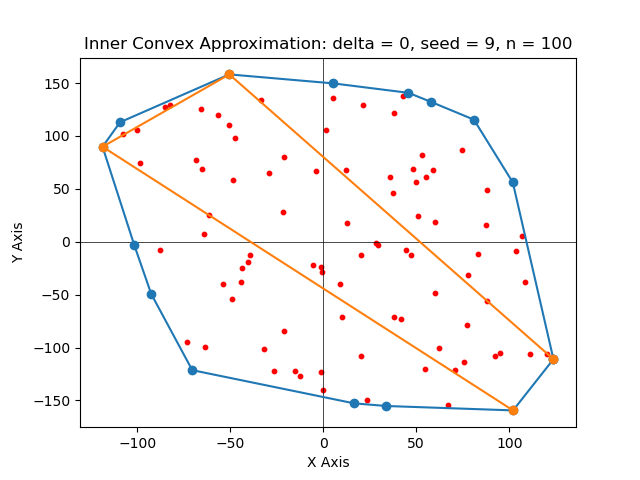
\includegraphics[width=300px]{./inner_cv_delta0.png}
		\caption{Inner Convex Approximation với delta = 0.}
		\label{inner_cv_delta0}
	\end{center}
\end{figure} 
\begin{figure}[ht!]
	\begin{center}
		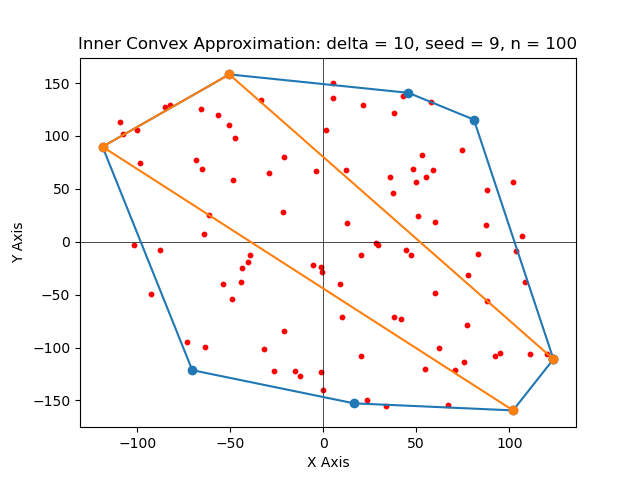
\includegraphics[width=300px]{./inner_cv_delta10.png}
		\caption{Inner Convex Approximation với delta = 10.}
		\label{inner_cv_delta10}
	\end{center}
\end{figure} 
\begin{figure}[ht!]
	\begin{center}
		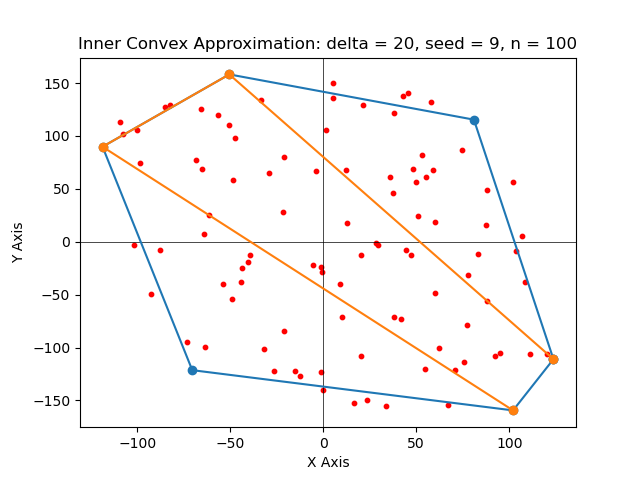
\includegraphics[width=300px]{./inner_cv_delta20.png}
		\caption{Inner Convex Approximation với delta = 20.}
		\label{inner_cv_delta20}
	\end{center}
\end{figure} 

\chapter{Thực nghiệm và kết quả}

Chương này trình bày cách thức triển khai của đồ án: khởi tạo môi trường chạy, lấy tập dữ liệu DOTA, chuyển đổi thuật toán từ mã Python sang mã c++, thay thế thuật toán mới cho thuật toán cũ, cấu hình file config để thực hiện huấn luyện, một vài kết quả số.
\section{Khởi tạo môi trường chạy} 

Môi trường được sử dụng trong đồ án: Linux, bản phân phối Ubuntu 20.04.06 LTS, sử dụng 2 máy có thông số khác nhau để chạy: máy laptop GTX 1650 4GB RAM, máy pc RTX 3060 12GB RAM. CUDA Toolkit 11.6 đã cài đặt CUDNN.

Do code trong paper Beyound Bounding Box đã không còn tương thích với phiên bản Mmcv \cite{mmcv} hiện đại, em đã chuyển qua sử dụng thư viện Mmrotate \cite{zhou2022mmrotate}, một thư viện mới được xây dựng vài tháng gần đây, có triển khai lại paper trên như là một bộ phát hiện mới, có tên là CFA.\\
 Thực hiện tải về các thư viện Mmcv==1.7.1, Mmdetection==2.28.2 và Mmrotate==0.3.4. Riêng 2 thư viện Mmcv và Mmrotate thực hiện clone repo về và xây dựng thư viện từ nguồn (build from source) theo như tài liệu của OpenMmlab.\\

OpenMmlab là một dự án mã nguồn mở phục vụ cho nghiên cứu học thuật và ứng dụng công nghiệp, bao gồm nhiều chủ đề nghiên cứu trong lĩnh vực thị giác máy tính như: phân loại hình ảnh, phát hiện mục tiêu, phân đoạn mục tiêu, tạo hình ảnh siêu phân giải, và nhiều hơn nữa.

OpenMmlab đã phát hành hơn 30 thư viện thị giác, đã triển khai hơn 300 thuật toán, và chứa hơn 2000 mô hình được huấn luyện trước.

Thư viện Mmcv đóng vai trò cung cấp các phép toán hỗ trợ ở mức thấp (sử dụng code CUDA c++ để lập trình tính toán cho card đồ hoạ). Thư viện Mmdetection \cite{mmdetection} là một bộ thư viện chủ đạo của phòng nghiên cứu OpenMmlab, cung cấp nền tảng để xây dựng tiếp một nhánh khác đó chính là thư viện Mmrotate. 

Mmdetection là một hộp công cụ phát hiện đối tượng chứa tập hợp các phương pháp phát hiện đối tượng phong phú, phân đoạn các thể hiện và phân đoạn toàn cảnh, cũng như các thành phân liên quan và các mô đun.

Mmrotate là một nhánh mới được xây dựng từ Mmdetection, là một hộp công cụ phát hiện đối tượng xoay dựa trên Pytorch. Nó cũng là một phần của các dự án OpenMMlab.

\begin{figure}[ht!]
	\begin{center}
		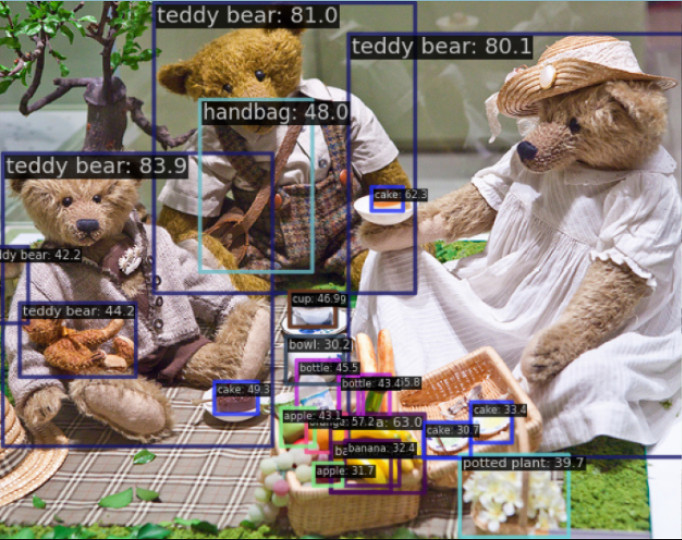
\includegraphics[width=250px]{./demo_mmrotate_result.jpg}
		\caption{Minh hoạ kết quả hình ảnh output của thư viện Mmrotate.}
		\label{demo_mmrotate_result}
	\end{center}
\end{figure} 

\section{Tập dữ liệu DOTA} 

Tập dữ liệu được sử dụng trong đồ án chính là tập dữ liệu DOTA v1.0. Tập dữ liệu DOTA được thu thập từ nền tảng Google Earth, GF-2 và vệ tinh JL-1 được cung cấp bởi Trung tâm Trung quốc nghiên cứu dữ liệu vệ tinh và ứng dụng, và các hình ảnh trên không được cung cấp bởi CycloMedia B.V. DOTA bao gồm các ảnh RGB và các ảnh mức xám. Tất cả các ảnh đều được lưu trữ dưới định dạng png. Tập dữ liệu DOTA có 3 phiên bản: v1.0, v1.5 và v2.0. Riêng tập dữ liệu v1.0 đã được chia sẵn các tập train, test, val.

Danh mục các class trong tập DOTA v1.0 bao gồm: plane, ship, storage tank, baseball diamond, tennis court, basketball court, ground track field, harbor, bridge, large vehicle, small vehicle, helicopter, roundabout, soccer ball field and swimming pool. (Hình \ref{minh_hoa_hop_bao_dota})

Mỗi đối tượng được gán nhãn bởi một hộp bao có hướng (oriented bounding box - OBB), được ký hiệu là: $(x_1, y_1, x_2, y_2, x_3, y_3, x_4, y_4)$. Trong đó $(x_i, y_i)$ biểu thị đỉnh thứ i của OBB. Các đỉnh được sắp xếp theo chiều kim đồng hồ. Ảnh \ref{minh_hoa_hop_bao_dota} minh hoạ trực quan các nhãn. Điểm màu vàng đại diện cho điểm bắt đầu, có nghĩa là: a) góc trái của máy bay, b) góc trái trên cùng của một phương tiện to, c) trung tâm của một sân bóng chày.

Mỗi một thể hiện trong file nhãn có thêm một danh mục (category) và độ khó (difficult) biểu thi liệu thể hiện này có khó nhận diện hay không (1 là khó, 0 là không khó). Các nhãn của một ảnh được lưu trong một file text với cùng tên file. Mỗi dòng trong file đại diện cho một thể hiện. Dưới đây là ví dụ 1 đoạn nội dung trong 1 file annotations:\\
717.0 76.0 726.0 78.0 722.0 95.0 714.0 90.0 small-vehicle 0  \\
737.0 82.0 744.0 84.0 739.0 101.0 731.0 98.0 small-vehicle 0 \\
658.0 242.0 648.0 237.0 657.0 222.0 667.0 225.0 small-vehicle 1 \\
735.0 122.0 754.0 129.0 750.0 136.0 733.0 128.0 small-vehicle 0 \\
773.0 137.0 788.0 144.0 784.0 151.0 770.0 144.0 small-vehicle 0 \\
809.0 153.0 827.0 161.0 823.0 168.0 806.0 160.0 small-vehicle 0 \\
696.0 122.0 705.0 124.0 697.0 141.0 691.0 137.0 small-vehicle 0 \\
707.0 126.0 714.0 130.0 706.0 145.0 700.0 141.0 small-vehicle 0 \\
711.0 140.0 718.0 141.0 712.0 157.0 706.0 154.0 small-vehicle 1 \\
924.0 113.0 926.0 106.0 945.0 115.0 942.0 122.0 small-vehicle 0 \\
935.0 95.0 939.0 88.0 955.0 97.0 950.0 104.0 small-vehicle 1 \\

\begin{figure}[ht!]
	\begin{center}
		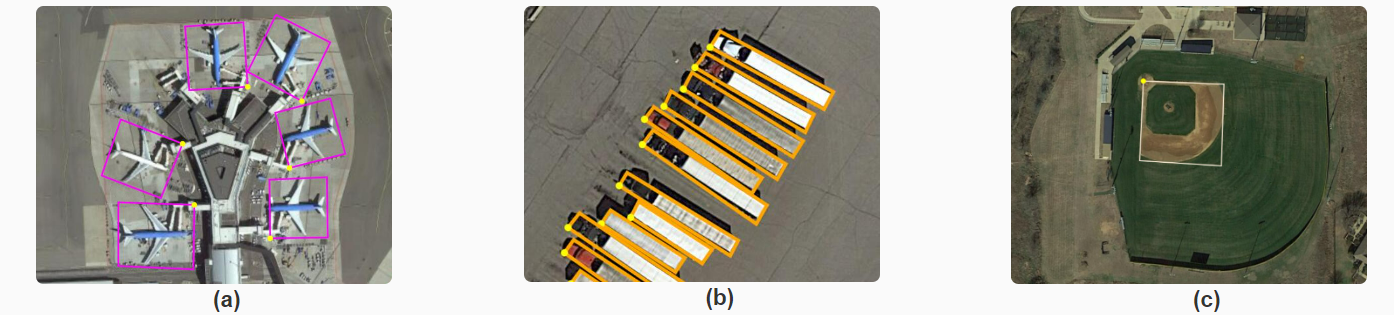
\includegraphics[width=445px]{./minh_hoa_hop_bao_dota.jpg}
		\caption{Minh hoạ nhãn hộp bao có hướng của tập dữ liệu DOTA.}
		\label{minh_hoa_hop_bao_dota}
	\end{center}
\end{figure} 
\section{Cách thức thay thế thuật toán}

Sau khi download được tập dữ liệu DOTA về máy, thực hiện tiền xử lý dữ liệu. Ta cần để cấu trúc dữ liệu dưới dạng cây như sau:
\dirtree{%
	.1 data.
	.2 DOTA.
	.3 train.
	.4 images.
	.5 P001.png.
	.5 P003.png.
	.5 \ldots.
	.4 labelTxt.
	.5 P001.txt.
	.5 P003.txt.
	.5 \ldots.
	.3 val.
	.4 images.
	.5 P000.png.
	.5 P002.png.
	.5 \ldots.
	.4 labelTxt.
	.5 P000.txt.
	.5 P002.txt.
	.5 \ldots.
	.3 test.
	.4 images.
	.5 P004.png.
	.5 P005.png.
	.5 \ldots.
	.4 test\_info.json.
}

Mở terminal rồi điều hướng vào thư mục gốc, thực hiện các lệnh sau:

\begin{lstlisting}[language=bash, caption={Câu lệnh để split ảnh trong tập dữ liệu DOTA},
basicstyle=\fontsize{11}{13}\selectfont,
keywordstyle=\bfseries,
label={lst:command-line}]
$ python tools/data/dota/split/img_split.py --base-json
tools/data/dota/split/split_configs/ss_trainval.json
$ python tools/data/dota/split/img_split.py --base-json
tools/data/dota/split/split_configs/ss_test.json
	
\end{lstlisting}


 Sử dụng lệnh để chia ảnh ra với 8 process, kích thước ảnh 1024 pixels, overlaps 200. Sau khi chia ta có cây thư mục của tập dữ liệu như sau:\\

\dirtree{%
	.1 data.
	.2 DOTA.
	.2 split\_ss\_dota.
	.3 trainval.
	.4 images.
	.5 P0000\_\_1024\_\_0\_\_\_0.png.
	.5 P0000\_\_1024\_\_0\_\_\_824.png.
	.5 P0000\_\_1024\_\_0\_\_\_1648.png.
	.5 ....
	.4 annfiles.
	.5 P0000\_\_1024\_\_0\_\_\_0.txt.
	.5 P0000\_\_1024\_\_0\_\_\_824.txt.
	.5 P0000\_\_1024\_\_0\_\_\_1648.txt.
	.5 ....
}



Tiếp theo thực hiện cài đặt miniconda, một phiên bản thu gọn của Anaconda. Sau đó chạy các câu lệnh sau:

\begin{lstlisting}[language=bash, caption={Câu lệnh để split ảnh trong tập dữ liệu DOTA},
	basicstyle=\fontsize{11}{13}\selectfont,
	keywordstyle=\bfseries,
	label={lst:command-line}]

$ conda create -n mmrotate_v26_beta1 --no-default-packages \
python==3.9 -y 
$ conda activate mmrotate_v26_beta1 
$ conda config --add channels conda-forge 
$ conda install pytorch==1.12.1 torchvision==0.13.1\ 
torchaudio==0.12.1 \
cudatoolkit=11.6 -c pytorch -c conda-forge 
$ cd mmcv
$ git checkout v1.7.1
$ pip install -r requirements/optional.txt 
$ Mmcv_WITH_OPS=1 pip install -e . -v 
$ pip install mmdet==2.28.2 
$ cd ../mmrotate 
$ git checkout v0.3.4
$ pip install -v -e . 
$ conda install packaging 
$ conda install scipy 
$ conda install python-dateutil
$ pip install future tensorboard
	
\end{lstlisting}


Ta cần phải thay thế code thuật toán mới vào thuật toán Jarvis. Để thay thế được ta cần phải thay thế vào thư viện mmcv, để thay thế 2 hàm Jarvis và Jarvis\_and\_index. Hai hàm hày có đầu vào là một mảng các Point tên là in\_poly đại diện cho số điểm cần tìm bao lồi, n\_poly đại diện cho số lượng phần tử trong mảng in\_poly. Đầu tiên thay thế bằng thuật toán Outer Convex Approximation thứ nhất. Thuật toán này có code Python như sau:

Một hàm khác cần thay thế là Jarvis\_and\_index(). Hàm này tương tự hàm Jarvis, nhưng bảo toàn thứ tự của các điểm trong bao lồi khi chúng còn là một tập hợp các điểm. Ta thêm vào đoạn code này phần đầu của hàm Jarvis\_and\_index():

Tiếp theo ta thêm đoạn code tương tự đoạn code Jarvis bên trên. Cuối cùng ta thêm đoạn code sau đây để lấy được chỉ số của các điểm nằm trên bao lồi trong tập điểm gốc:


\begin{lstlisting}[language=python, caption={Câu lệnh để split ảnh trong tập dữ liệu DOTA},
	basicstyle=\fontsize{11}{13}\selectfont,
	keywordstyle=\bfseries,
	label={lst:command-line}]
from mmcv import Config
from mmrotate.datasets.builder import ROTATED_DATASETS
from mmrotate.datasets.dota import DOTADataset


@ROTATED_DATASETS.register_module()
class CustomDotaDataset(DOTADataset):
"""SAR ship dataset for detection."""
CLASSES = ('plane', 'baseball-diamond', 
			'bridge', 'ground-track-field',
			'small-vehicle', 'large-vehicle',
			'ship', 'tennis-court',
			'basketball-court', 'storage-tank'
			, 'soccer-ball-field',
			'roundabout', 'harbor',
			'swimming-pool', 'helicopter')
cfg = Config.fromfile('./configs/cfa/cfa_r50_fpn_40e_dota_oc.py')
from mmdet.apis import set_random_seed

cfg.dataset_type = 'CustomDotaDataset'
cfg.data_root = 'data/split_ss_dota/'

cfg.data.test.type = 'CustomDotaDataset'
cfg.data.test.data_root = 'data/split_ss_dota/'
cfg.data.test.ann_file = 'test/annfiles/'
cfg.data.test.img_prefix = 'test/images/'

cfg.data.train.type = 'CustomDotaDataset'
cfg.data.train.data_root = 'data/split_ss_dota/'
cfg.data.train.ann_file = 'trainval/annfiles/'
cfg.data.train.img_prefix = 'trainval/images/'

cfg.data.val.type = 'CustomDotaDataset'
cfg.data.val.data_root = 'data/split_ss_dota/'
cfg.data.val.ann_file = 'trainval/annfiles/'
cfg.data.val.img_prefix = 'trainval/images/'

cfg.work_dir = './results'
cfg.log_config.interval = 50

cfg.evaluation.interval = 5
cfg.checkpoint_config.interval = 1

# Set seed thus the results are more reproducible
cfg.seed = 0
set_random_seed(0, deterministic=False)
cfg.gpu_ids = range(1)
cfg.device='cuda'

import os.path as osp
import os
import mmcv
from mmdet.datasets import build_dataset
from mmdet.models import build_detector
from mmdet.apis import train_detector

import torch
torch.cuda.empty_cache()

# Build dataset
datasets = [build_dataset(cfg.data.train)]

# Build the detector
model = build_detector(
cfg.model, train_cfg=cfg.get('train_cfg'),
test_cfg=cfg.get('test_cfg'))
# Add an attribute for visualization convenience
model.CLASSES = datasets[0].CLASSES
mmcv.mkdir_or_exist(osp.abspath(cfg.work_dir))
train_detector(model, datasets,
cfg, distributed=False, validate=True)
	
\end{lstlisting}

Ta cần phải triển khai code của thuật toán Outer Convex Approximation và Inner Convex Approximation dưới dạng mã CUDA C++. CUDA (Compute Unified Device Architecture) C++ là một phần của môi trường lập trình CUDA, được phát triển bởi NVIDIA để hỗ trợ lập trình đa luồng trên GPU (Graphics Processing Unit). Mã CUDA C++ cung cấp một cách hiệu quả để triển khai và thực hiện các tác vụ tính toán song song trên GPU, giúp tận dụng sức mạnh tính toán lớn của các card đồ họa hiện đại.

Mã CUDA C++ đều được viết trong một chương trình C++ tiêu chuẩn, nhưng có thêm các mở rộng và đặc điểm cụ thể của CUDA để hỗ trợ lập trình song song trên GPU. Điều này giúp lập trình viên hiệu quả hóa ứng dụng của mình để sử dụng tối đa sức mạnh tính toán của GPU.

Hai thuật tóan mới đưa vào phải tuân theo đầu vào và đầu ra tương tự thuật toán Jarvis. Các tham số của thuật toán Jarvis là:\\ Jarvis(Point* in\_poly, int n\_poly){}\\ trong đó in\_poly là một mảng gồm 9 hoặc 18 phần tử Point(x, y) đại diện cho các điểm đặc trưng. Thuật toán Jarvis sẽ thay đổi phần tử trong mảng in\_poly, để trả về chỉ còn các phần tử Point của bao lồi, và thay đổi n\_poly thành số lượng các phần tử trên bao lồi. Ngoài ra còn một hàm Jarvis\_and\_index có các tham số đầu vào như sau: \\ Jarvis\_and\_index(Point* in\_poly, int n\_poly, int* point\_to\_convex\_index){}.\\ Hàm này tính toán tương tự như hàm Jarvis(), tuy nhiên trả về thêm một mảng chỉ số của các phần tử gốc trước khi mảng in\_poly bị thay đổi. Mảng này được khởi tạo toàn bộ giá trị bằng -1. Vậy hai hàm của từng thuật toán mới sẽ được thay vào hai hàm CUDA trên và hoạt động tương tự thuật toán Jarvis.

Tóm lại trong chương 3 này trình bày cách thức để tạo môi trường huấn luyện, cách thức xử lý data trước khi đem vào huấn luyện, cuối cùng là cách thức để thay thế thuật toán Jarvis bằng thuật toán mới sao cho quá trình huấn luyện có thể được thực thi.

\chapter{Một số kết quả tính toán }
\begin{figure}
	\centering
	\includegraphics[width=16cm]{../slide-do-an/detection_performance_on_DOTA}
	\caption{Kết quả của bộ phát hiện CFA thực hiện trên tập dữ liệu DOTA khi so sánh với các bộ phát hiện khác}
	\label{detectionperformanceondota}
\end{figure}

Bộ phát hiện CFA được so sánh với các bộ phát hiện tốt nhất trên tập dữ liệu DOTA với nhiệm vụ xác định hộp bao có hướng. Vì là một bộ phát hiện không dùng anchor, CFA vượt trội hơn bộ phát hiện DRN mới nhất khoảng 5.97\% (76.67\% vs 70.70\%), một khoảng cách khá lớn. Cụ thể, trong các lớp SV, LV, RA, HA và SP, CFA vượt trội hơn 7.75\% (81.23\% vs. 73.48\%), 10.27\% (80.96\% vs. 70.69\%), 11.53\% (69.94\% vs. 58.41\%),7.90\%(75.52\% vs. 67.62\%), and 12.16\% (80.76\% vs. 68.60\%). Nguyên nhân ở đây có thể là do dạnh mục các đối tượng có hình dạng bất thường, và CFA sử dụng biểu diễn bao lồi có thể thích nghi tốt hơn với những đối tượng có bố cục và hướng bất thường. Vì là bộ phát hiện anchor-free, CFA có thể so sánh nếu không muốn nói là tốt hơn các bộ phát hiện base-detector như RoI-Transformer, SCRDet, Gliding Vertex và CSL.

Hình \ref{convexhullevolutionduringtraining} cho thấy quá trình phát triển của bao lồi. Có thể thấy sau khi khởi tạo, bao lồi dần dần tiếp cận tới hộp bao thực tế (ground-truth). Phần lớn các điểm đặc trưng (feature point), đều nằm bên trong phần mở rộng của đối tượng (phần được bao bởi grouth-truth). 

Trong hình \ref{heatmapcomparisionofcfa} so sánh bộ phát hiện khi có và không có chức năng anti-feature aliasing. Với việc thích ứng đặc trưng, biểu đồ nhiệt tại vị trí các đối tượng nằm dày đặc được chia tách rõ ràng. Điều này xác nhận sự ảnh hưởng của tính năng feature anti-aliasing của bộ phát hiện CFA.

Thực hiện một vài nghiên cứu về các siêu tham số và các module khác, CFA cũng thu được các kết quả như sau:

\textbf{CIoU}: CIoU phản ánh mức độ ảnh hưởng của mức độ chồng lấp của hộp dự đoán và hộp bao thực tế. Tối thiểu hóa hàm loss CIoU sẽ cải thiện được hộp bao dự đoán. Bảng \ref{comparecioulosswithl1loss} thực hiện so sánh hàm loss CIoU và hàm loss Smoothed-L1, CIoU đã cải thiện chỉ số mAP lên 0.95\% (66.30\% và 65.35\%).

\begin{figure}
	\centering
	\includegraphics[width=6cm]{../slide-do-an/compare_CIoU_loss_with_L1_loss}
	\caption{So sánh hàm loss CIoU và hàm loss Smoothed-L1.}
	\label{comparecioulosswithl1loss}
\end{figure}
 
 
\textbf{Convex-Hull Generation}: Bằng cách mô hình hóa đối tượng thành dạng bao lồi, giúp giảm được hiện tượng feature aliasing từ cả phần nền và các đối tượng lân cận. Trong quá trình huấn luyện, bao lồi được sinh ra và thích ứng với phần mở rộng của đối tượng. Trong bảng \ref{fig:nghiencuucatbocuacacmodule} và hình \ref{fig:evaluationofhyperparameterandmodules}b, bằng cách sử dụng phương pháp phân chia tập bao lồi, CFA cải thiện được hiệu suất bộ phát hiện lên 1.52\% (69.70\% và 68.18\%), xác nhận nguyên tắc đạo hàm nhất quán với feature alasing. Ở hình \ref{fig:evaluationofhyperparameterandmodules}d, xác nhận rằng khởi tạo 6 bao lồi với mỗi mức feature pyramid(\textit{I}=6) với mỗi tập hợp bao lồi sẽ đạt được hiệu suất tốt nhất.

\textbf{Anti-aliasing Coefficient}: Bằng cách sử dụng hệ số khử đặc trưng răng cưa (FA-A), việc thích ứng bao lồi với nhiều đối tượng được triển khai và hiệu suất được cải thiện bởi 0.43\% (70.13\% và 69.70\%) với hệ số $\gamma$=0.75 ở hình \ref{fig:evaluationofhyperparameterandmodules}d. Nói chung, bộ phát hiện CFA đã cải thiện bộ phát hiện gốc lên 4.79\% mAP.


\begin{figure}
	\centering
	\includegraphics[width=12cm]{../slide-do-an/nghien_cuu_cat_bo_cua_cac_module}
	\caption{Nghiên cứu cắt bỏ của các module trong CFA. CGen là Convex hull Generation, FA-S là feature adaptation by set splitting, FA-A là Feature Adaptation với anti-aliasing. Mạng backbone được dùng là ResNet50.}
	\label{fig:nghiencuucatbocuacacmodule}
\end{figure}
\begin{figure}
	\centering
	\includegraphics[width=12cm]{../slide-do-an/evaluation_of_hyperparameter_and_modules}
	\caption{Đánh giá tham số và các modules. }
	\label{fig:evaluationofhyperparameterandmodules}
\end{figure}

\begin{figure}
	\centering
	\includegraphics[width=16cm]{../slide-do-an/convex_hull_evolution_during_training}
	\caption{Quá trình phát triển của bao lồi trong quá trình huấn luyện.}
	\label{convexhullevolutionduringtraining}
\end{figure}
\begin{figure}
	\centering
	\includegraphics[width=16cm]{../slide-do-an/heat_map_comparision_of_CFA}
	\caption{Biểu đồ nhiệt khi có thích nghi đặc trưng và không có thích nghi đặc trưng}
	\label{heatmapcomparisionofcfa}
\end{figure}

Trong quá trình thay mới thuật toán Convex Approximation, ta cần quan tâm đến các yếu tố sau:

Về vị trí cần thay hàm: Có hai hàm cần thay là Jarvis() và Jarvis\_and\_index().

Về bộ dataset sử dụng: Có hai bộ đó là bộ hoàn chỉnh và bộ có 1000 ảnh trainval, 500 ảnh test. Yêu cầu của lần huấn luyện là phải đi qua được 40 epoch.

Với mỗi yếu tố trên ta sẽ thử với nhiều lần, trong đó có các lần thử tiêu biểu như sau:

\section{Thay thế Outer Convex Approximation và huấn luyện sử dụng bộ dữ liệu đầy đủ}

Sử dụng thuật toán Outer Convex Approximation để thay thế vào hai hàm trên, sau đó cho thuật toán huấn luyện với bộ dữ liệu DOTA đã được chia cắt tỷ lệ ảnh.\\

\begin{figure}[ht!]
	\begin{center}
		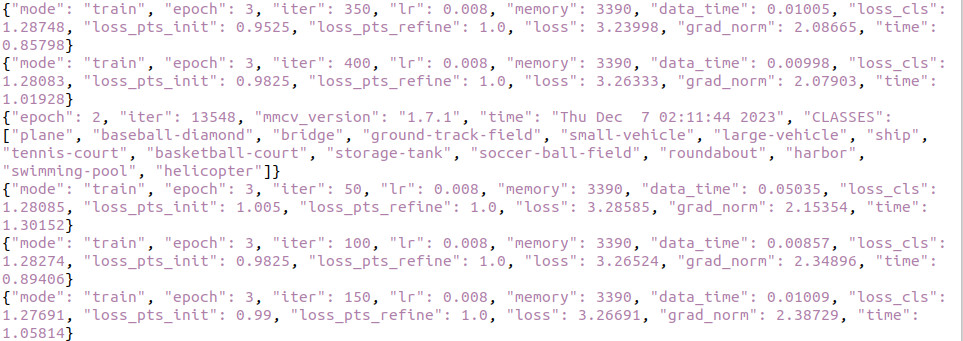
\includegraphics[width=450px]{./outer_fulldata_epoch3.JPG}
		\caption{Outer Convex Approximation sử dụng toàn bộ tập dữ liệu, sập tại epoch số 3.}
		\label{outer_fulldata_epoch3}
	\end{center}
\end{figure} 

\textbf{Kết quả huấn luyện}: Máy chạy tốt cho đến epoch thứ 3 báo lỗi illegal memory (Hình \ref{outer_fulldata_epoch3}). Dự đoán nguyên nhân do tính toán bị sai hoặc máy hết dung lượng. Thực hiện restart máy và cho chạy lại từ file checkpoint mới nhất, tuy nhiên kết quả vẫn tương tự và không chạy thêm được epoch nào.
\section{Thay thế Outer Convex Approximation và huấn luyện sử dụng dataset nhỏ}

\begin{figure}[ht!]
	\begin{center}
		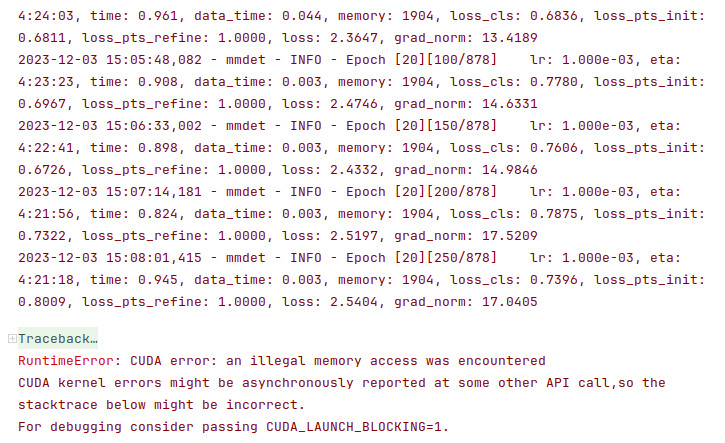
\includegraphics[width=450px]{./mmrotate8_1000p_epoch20.JPG}
		\caption{Outer Convex Approximation chạy với dataset nhỏ, sập tại epoch 20.}
		\label{mmrotate8_1000p_epoch20}
	\end{center}
\end{figure} 

\begin{figure}[ht!]
	\begin{center}
		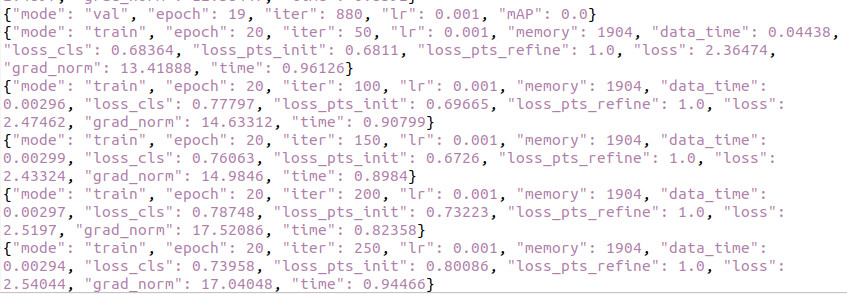
\includegraphics[width=450px]{./ket_qua_file_none_log_json.JPG}
		\caption{Outer Convex Approximation train với dataset nhỏ, sập tại epoch 20.}
		\label{ket_qua_file_none_log_json}
	\end{center}
\end{figure} 

Do cần có kết quả sớm để xem thuật toán có thực hiện được hay không, ta sẽ sử dụng với bộ dataset nhỏ hơn. Bộ dataset này được lấy từ bộ dataset đầy đủ với 1000 ảnh và nhãn dành cho tập trainval, 500 ảnh dành cho tập test. Kết quả là thuật toán chạy được đến epoch số 20 là bị sập, báo lỗi illigal memory (Hình \ref{mmrotate8_1000p_epoch20}). Ngoài ra quá trình huấn luyện thu được file checkpoint  và file log (Hình \ref{ket_qua_file_none_log_json}).

\section{Thay thế Outer Convex Approximation vào hàm Jarvis() và huấn luyện sử dụng dataset nhỏ}

Do nghi ngờ kết quả lỗi xuất hiện ở hàm Jarvis\_and\_index(), em chỉ thay thuật toán vào hàm Jarvis, tức là trong quá trình huấn luyện sẽ có sử dụng cả thuật toán Jarvis March và thuật toán Outer Convex Approximation. Kết quả quá trình huấn luyện diễn ra được thuận lợi, thuật toán chạy hết được 40 epochs mà không gặp lỗi gì. Tuy nhiên do bộ dataset quá nhỏ, cùng với giới hạn các class trong dataset bị mất cân bằng nên không sử dụng được kết quả này, chỉ có thể chứng minh được là thuật toán đã hoạt động được và cho kết quả chạy chính xác. Tuy nhiên kết luận này vẫn cần phải kiểm tra và xác minh lại tính chính xác khách quan hơn.

\begin{figure}[ht!]
	\begin{center}
		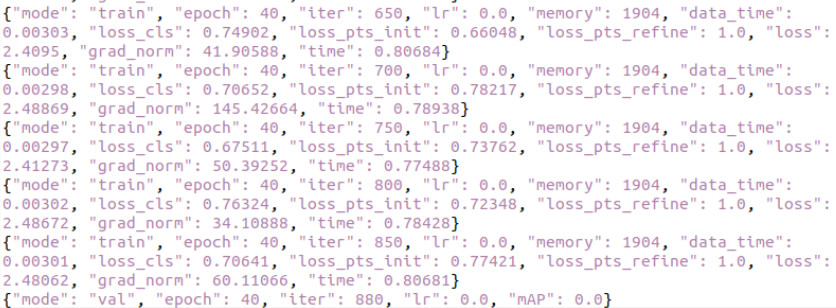
\includegraphics[width=450px]{./outer_just_javis_smalldata_40epoch.JPG}
		\caption{Outer Convex Approximation chỉ thay code ở hàm Jarvis, đạt được 40 epoch.}
		\label{outer_just_javis_smalldata_40epoch}
	\end{center}
\end{figure} 
\section{Thay thế Inner Convex Approximation và huấn luyện sử dụng toàn bộ dữ liệu đầy đủ}

\textbf{Kết quả}: Quá trình huấn luyện chạy thuận lợi cho đến epoch số 15, máy báo lỗi Illegal Memory, tức là lỗi truy cập vùng nhớ không hợp lệ.

\begin{figure}[ht!]
	\begin{center}
		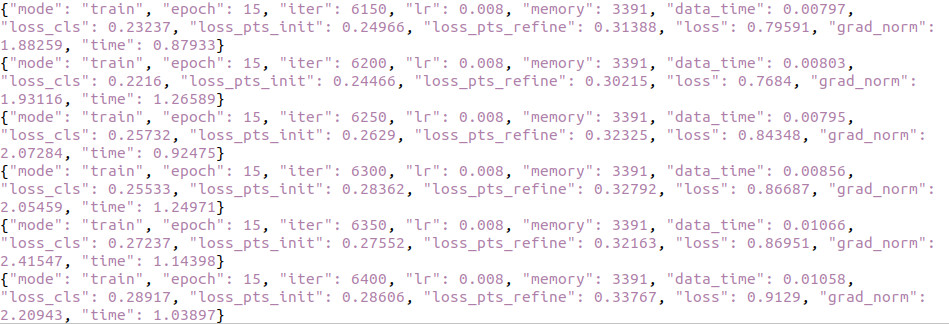
\includegraphics[width=450px]{./inner_fulldata_epoch15.JPG}
		\caption{Inner Convex Approximation train với toàn bộ dữ liệu, sập tại epoch số 15.}
		\label{inner_fulldata_epoch15}
	\end{center}
\end{figure} 
\section{Thay thế Inner Convex Approximation và huấn luyện sử dụng bộ dữ liệu nhỏ}

\textbf{Kết quả}: Máy chạy đến epoch số 20 báo lỗi Illegal Memory.

\begin{figure}[ht!]
	\begin{center}
		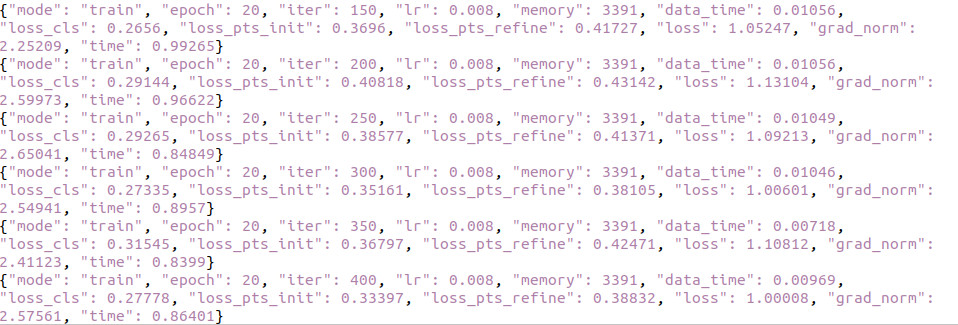
\includegraphics[width=450px]{./inner_smalldata_epoch20.JPG}
		\caption{Inner Convex Approximation train với bộ dữ liệu nhỏ hơn, sập tại epoch số 20.}
		\label{inner_smalldata_epoch20}
	\end{center}
\end{figure} 

\chapter*{{Kết luận}}
\addcontentsline{toc}{chapter}{\vspace*{-8pt} Kết luận}
Tóm lại trong đồ án này, em đã thực hiện các công việc sau:
\begin{itemize}
	\item Đọc và tìm hiểu tài liệu của bộ phát hiện CFA
	\item Chuẩn bị tập dữ liệu DOTA để cho vào huấn luyện
	\item Thực hiện chạy thử huấn luyện với tập dữ liệu DOTA như trong bài báo của CFA
	\item Viết mã CUDA C++ cho 2 thuật toán Outer Convex Approximation và Inner Convex Approximation
	\item Tìm cách thay thế hai thuật toán mới này vào thư viện Mmcv để có thể huẩn luyện mô hình
\end{itemize}

Trong tất cả các lần huấn luyện trên, chỉ có lần thử với bộ dataset nhỏ cùng với việc thay thế 1 nửa thuật toán là đáp ứng được quá trình training 40 epoch. Vì số lượng bộ dữ liệu không đảm bảo cho kết quả huấn luyện đúng, nên chỉ có thể kết luận rằng thuật toán mới có thể thay thế được vào bộ phát hiện, nhưng chưa thể sử dụng được kết quả. Có nhiều nguyên nhân khác nhau dẫn đến lỗi, nhưng nguyên nhân chính vẫn là chưa tìm hiểu đủ kiến thức cũng như kinh nghiệm trong công việc này.

Các khó khăn chính khi thực hiện đồ án: 
\begin{itemize}
	\item Tài liệu khó đọc
	\item Thiết lập môi trường cài đặt rất khó
	\item Mã CUDA C++ có vài điểm khác biệt so với mã C++ truyền thống. Việc này làm cho quá trình viết mã mới gặp nhiều khó khăn
	\item Khó debug được lỗi viết bằng mã CUDA C++. Gần như không thể xem log được thông tin gì. Cần phải sử dụng các kỹ thuật debug khác
\end{itemize}

Qua các lần training không thành công, em xin đề xuất hướng xử lý tiếp theo của đồ án:
\begin{itemize}
	\item Cần kiểm tra lại file config cấu hình training. Nếu file này cấu hình chưa đúng dẫn đến hiện tượng training giữa chừng thì bị lỗi.
	\item Xem xét lỗi Illegal Memory. Lỗi này là lỗi chính bắt gặp khi thực hiện train. Cần phải tìm hiểu kĩ hơn nữa về nguyên nhân của lỗi là do phần cứng hay phần mềm sinh ra.
	\item Cần tìm hiểu thêm về cách thư viện Mmrotate hoạt động. Đây là một thư viện lớn, có nhiều thuật ngữ và thuật toán khó hiểu. 
	\item Tìm hiểu thêm nhiều tài liệu về bài toán phát hiện đối tượng nói riêng, cũng như trong lĩnh vực trí tuệ nhân tạo nói chung.
\end{itemize}

Trong quá trình làm đồ án tốt nghiệp, em đã có cơ hội được trải nghiệm chuyên ngành AI cũng như được thử sức qua các công nghệ nhận diện ảnh mới nhất. Em đã tích luỹ được những kinh nghiệm về kiến thức trong công việc cũng như các kỹ năng mềm trong xử lý các công việc liên quan đến hệ điều hành linux, cách triển khai một dự án trí tuệ nhân tạo, cách tìm hiểu thông tin từ các tài liệu chính thống.
 
Em được rèn luyện kỹ năng giải quyết các công việc con, cách tương tác với người khác để trao đổi kiến thức, từ đó rút ngắn công sức và thời gian. Đồng thời em cũng được áp dụng lại các kiến thức đã được học từ các môn trên trường vào đồ án thực tế này.
\bibliographystyle{plain}
\bibliography{trichdan}
\end{document}
 
